\documentclass[a4paper]{article}
% basics
\usepackage[utf8]{inputenc}
\usepackage[T1]{fontenc}
\usepackage{fontspec} % Pour les accents de Tomáš Kaiser
% \usepackage{textcomp}
% \usepackage{url}
\usepackage{graphicx}
\usepackage{float}
% \usepackage{booktabs}
% \usepackage[shortlabels]{enumitem}
% \usepackage{parskip}
% \usepackage{emptypage}
% \usepackage{subcaption}
% \usepackage{multicol}
\usepackage[usenames,dvipsnames]{xcolor}
% \usepackage{cmbright}
\usepackage[shortlabels]{enumitem}
% \setlist[itemize,1]{label={\color{gray}\small \textbullet}}
\usepackage{amsmath, amsfonts, mathtools, amsthm, amssymb}
\usepackage{mathrsfs}
% \usepackage{cancel}
% \usepackage{bm}
\newcommand\N{\ensuremath{\mathbb{N}}}
\newcommand\R{\ensuremath{\mathbb{R}}}
\newcommand\Z{\ensuremath{\mathbb{Z}}}
\renewcommand\O{\ensuremath{\emptyset}}
\newcommand\Q{\ensuremath{\mathbb{Q}}}
\newcommand\C{\ensuremath{\mathbb{C}}}
\DeclareMathOperator{\sgn}{sgn}
% \usepackage{systeme}
\let\svlim\lim\def\lim{\svlim\limits}
\let\implies\Rightarrow
\let\impliedby\Leftarrow
\let\iff\Leftrightarrow
\let\epsilon\varepsilon
% \usepackage{stmaryrd} % for \lightning
% \newcommand\contra{\scalebox{1.1}{$\lightning$}}
% \let\phi\varphi


% correct
\definecolor{correct}{HTML}{009900}
\newcommand\correct[2]{\ensuremath{\:}{\color{red}{#1}}\ensuremath{\to }{\color{correct}{#2}}\ensuremath{\:}}
\newcommand\green[1]{{\color{correct}{#1}}}



% horizontal rule
\newcommand\hr{
    \noindent\rule[0.5ex]{\linewidth}{0.5pt}
}


% hide parts
\newcommand\hide[1]{}



% si unitx
\usepackage{siunitx}
\sisetup{locale = FR}
% \renewcommand\vec[1]{\mathbf{#1}}
\newcommand\mat[1]{\mathbf{#1}}


% tikz
\usepackage{tikz}
\usepackage{tikz-cd}
\usetikzlibrary{intersections, angles, quotes, calc, positioning}
\usetikzlibrary{arrows.meta}
%\usepackage{pgfplots}
%\pgfplotsset{compat=1.13}


\tikzset{
    force/.style={thick, {Circle[length=2pt]}-stealth, shorten <=-1pt}
}

% theorems
\usepackage{thmtools}
\usepackage[framemethod=TikZ]{mdframed}
\mdfsetup{skipabove=1em,skipbelow=0em, innertopmargin=5pt, innerbottommargin=6pt}


\theoremstyle{definition}

\makeatletter


\declaretheoremstyle[
    headfont=\bfseries\sffamily\color{ForestGreen!70!black}, bodyfont=\normalfont,
    mdframed={
        linewidth=2pt,
        rightline=false, topline=false, bottomline=false,
        linecolor=ForestGreen, backgroundcolor=ForestGreen!5,
    }
]{thmgreenbox}

\declaretheoremstyle[
    headfont=\bfseries\sffamily\color{NavyBlue!70!black}, bodyfont=\normalfont,
    mdframed={
        linewidth=2pt,
        rightline=false, topline=false, bottomline=false,
        linecolor=NavyBlue, backgroundcolor=NavyBlue!5,
    }
]{thmbluebox}

\declaretheoremstyle[
    headfont=\bfseries\sffamily\color{NavyBlue!70!black}, bodyfont=\normalfont,
    mdframed={
        linewidth=2pt,
        rightline=false, topline=false, bottomline=false,
        linecolor=NavyBlue
    }
]{thmblueline}

\declaretheoremstyle[
    headfont=\bfseries\sffamily\color{RawSienna!70!black}, bodyfont=\normalfont,
    mdframed={
        linewidth=2pt,
        rightline=false, topline=false, bottomline=false,
        linecolor=RawSienna, backgroundcolor=RawSienna!5,
    }
]{thmredbox}

\declaretheoremstyle[
    headfont=\bfseries\sffamily\color{RawSienna!70!black}, bodyfont=\normalfont,
    numbered=no,
    mdframed={
        linewidth=2pt,
        rightline=false, topline=false, bottomline=false,
        linecolor=RawSienna, backgroundcolor=RawSienna!1,
    },
    qed=\qedsymbol
]{thmproofbox}

\declaretheoremstyle[
    headfont=\bfseries\sffamily\color{NavyBlue!70!black}, bodyfont=\normalfont,
    numbered=no,
    mdframed={
        linewidth=2pt,
        rightline=false, topline=false, bottomline=false,
        linecolor=NavyBlue, backgroundcolor=NavyBlue!1,
    },
]{thmexplanationbox}
\declaretheorem[style=thmgreenbox, numbered=no, name=Définition]{definition}
\declaretheorem[style=thmbluebox, numbered=no, name=Exemple]{eg}
\declaretheorem[style=thmbluebox, numbered=no, name=Exercice]{ex}
\declaretheorem[style=thmredbox, name=Proposition]{prop}
\declaretheorem[style=thmredbox, numbered=no, name=Théorème]{theorem}
\declaretheorem[style=thmredbox, numbered=no,name=Lemme]{lemma}
\declaretheorem[style=thmredbox, numbered=no, name=Corollaire]{corollary}

\declaretheorem[style=thmproofbox, name=Preuve]{replacementproof}
\renewenvironment{proof}[1][\proofname]{\vspace{-10pt}\begin{replacementproof}}{\end{replacementproof}}

\declaretheorem[style=thmexplanationbox, name=Proof]{tmpexplanation}
\newenvironment{explanation}[1][]{\vspace{-10pt}\begin{tmpexplanation}}{\end{tmpexplanation}}

\makeatother


\declaretheorem[style=thmblueline, numbered=no, name=Remarque]{remark}
\declaretheorem[style=thmblueline, numbered=no, name=Note]{note}

\newtheorem*{uovt}{UOVT}
\newtheorem*{notation}{Notation}
\newtheorem*{previouslyseen}{As previously seen}
\newtheorem*{problem}{Problem}
\newtheorem*{observe}{Observe}
\newtheorem*{property}{Property}
\newtheorem*{intuition}{Intuition}


\usepackage{etoolbox}
\AtEndEnvironment{vb}{\null\hfill$\diamond$}%
\AtEndEnvironment{intermezzo}{\null\hfill$\diamond$}%
% \AtEndEnvironment{opmerking}{\null\hfill$\diamond$}%

% http://tex.stackexchange.com/questions/22119/how-can-i-change-the-spacing-before-theorems-with-amsthm
% \def\thm@space@setup{%
%   \thm@preskip=\parskip \thm@postskip=0pt
% }

\newcommand{\oefening}[1]{%
    \def\@oefening{#1}%
    \subsection*{Oefening #1}
}

\newcommand{\suboefening}[1]{%
    \subsubsection*{Oefening \@oefening.#1}
}

\newcommand{\exercise}[1]{%
    \def\@exercise{#1}%
    \subsection*{Exercise #1}
}

\newcommand{\subexercise}[1]{%
    \subsubsection*{Exercise \@exercise.#1}
}


\usepackage{xifthen}

\def\testdateparts#1{\dateparts#1\relax}
\def\dateparts#1 #2 #3 #4 #5\relax{
    \marginpar{\small\textsf{\mbox{#1 #2 #3 #5}}}
}

\def\@lesson{}%
\newcommand{\lesson}[3]{
    \ifthenelse{\isempty{#3}}{%
        \def\@lesson{Lecture #1}%
    }{%
        \def\@lesson{Lecture #1: #3}%
    }%
    \subsection*{\@lesson}
    \testdateparts{#2}
}

% \renewcommand\date[1]{\marginpar{#1}}


% fancy headers
\usepackage{fancyhdr}


\makeatother




% notes
% \usepackage{todonotes}
\usepackage{tcolorbox}

\tcbuselibrary{breakable}
\newenvironment{verbetering}{\begin{tcolorbox}[
    arc=0mm,
    colback=white,
    colframe=green!60!black,
    title=Opmerking,
    fonttitle=\sffamily,
    breakable
]}{\end{tcolorbox}}

\newenvironment{noot}[1]{\begin{tcolorbox}[
    arc=0mm,
    colback=white,
    colframe=white!60!black,
    title=#1,
    fonttitle=\sffamily,
    breakable
]}{\end{tcolorbox}}




% figure support
% \usepackage{import}
% \usepackage{pdfpages}
% \usepackage{transparent}
% \newcommand{\incfig}[1]{%
%     \def\svgwidth{\columnwidth}
%     \import{./figures/}{#1.pdf_tex}
% }

% algorithms
\usepackage{algorithm}
\usepackage{algpseudocode}
% Options possibles : 10pt, 11pt, 12pt (taille de la fonte)
%                     oneside, twoside (recto simple, recto-verso)
%                     draft, final (stade de développement)
\usepackage[french]{babel}  
\usetikzlibrary{arrows,shapes,positioning}
\usepackage{float}
\definecolor{myblue}{RGB}{85,114,193}
\tikzset{Dotted/.style={
    line width=1pt,
    dash pattern=on 0.01\pgflinewidth off #1\pgflinewidth,line cap=round,
    shorten >=0.3em,shorten <=0.3em},
    Dotted/.default=5}
\usetikzlibrary{arrows.meta,calc,positioning,shapes,arrows}
%\usepackage{pdflscape}
\usepackage{geometry}
\usepackage[backref=true]{biblatex}
\addbibresource{biblio.bib}
\usepackage{csquotes}
\usepackage[colorlinks=true, urlcolor=blue,urlbordercolor={0 1 1}]{hyperref}
\hypersetup{
	pdftitle={Stratégies de résolution du problème du flot maximum}
}
\usepackage{datetime}
\usepackage{numprint}
\usepackage{listings}
\usepackage{tabto}
\usepackage{tcolorbox}
\usepackage{xcolor}
\usepackage{graphicx}
\usepackage{subcaption}
\lstset{
  basicstyle=\ttfamily\small,
  frame=single,
  columns=fullflexible
}

\newcommand{\setImportantColor}[1]{
	\renewmdenv[
	linewidth=2pt,
	linecolor=#1,
	leftline=true,
	topline=false,
	bottomline=false,
	rightline=false
	]{importantinfo}
}

\newdate{frontpagedate}{26}{05}{2025} 
\begin{document}
\pagenumbering{gobble} 
\begin{center}
\vspace{2cm}
%\textsc{ Oregon State University}\\[1.5cm]

\includegraphics[width=0.4\textwidth]{UM1.jpg}~\\[1cm]
\vspace{2cm}

% Title
\hrule
\vspace{.5cm}
{\huge\bfseries{Stratégies de résolution du problème du flot maximum\par}} % title of the report
\vspace{.5cm}

\hrule
\vspace{1.5cm}

\textsc{\textbf{Auteurs}}\\
\vspace{.5cm}
\centering

% add your name here
Cédric Audie\\
Marie Dalenc\\
Julien Lahoz\\
Adrien Martinelli


\vspace{1cm}

\textsc{\textbf{Encadrant}}\\
\vspace{.5cm}
\centering

% add your name here
Rodolphe Giroudeau

\vspace{4cm}

\centering \displaydate{frontpagedate} % Dags dato
\end{center}
\newpage
\begin{abstract}	
Le problème du flot maximum est un problème d'optimisation combinatoire classique en informatique et en recherche opérationnelle. Étant donné un réseau de flot, l'objectif est de déterminer la quantité maximale de flot qui peut être envoyée d'une source à un puits, tout en respectant les contraintes de capacité des arcs et de conservation du flot. Ce problème a de nombreuses applications pratiques, notamment dans la planification logistique, les réseaux de transport et les réseaux de communication. 

Dans ce travail, nous comparons différentes méthodes de résolution du problème du flot maximum.  Nous étudions les algorithmes classiques tels que Ford-Fulkerson, Edmonds-Karp, Poussage-Réétiquetage et Dinic, ainsi que des approches basées sur la programmation linéaire. Nous mettons en œuvre ces algorithmes et les testons sur un ensemble de graphes générés aléatoirement. Nous analysons les performances de chaque méthode en termes de complexité théorique et de temps d'exécution pratique. 
\end{abstract}
\newpage
{\hypersetup{hidelinks}
\tableofcontents
}
\pagenumbering{arabic} 
\newpage
\pagestyle{headings}
\section{Introduction}
Le problème du flot maximum est l’un des problèmes fondamentaux en algorithmique et en recherche opérationnelle. Il consiste à trouver, dans un réseau orienté avec des capacités sur les arcs, le flot de valeur maximale entre une source et un puits, tout en respectant les contraintes de capacité et de conservation des flots.

Depuis plusieurs décennies, de nombreux algorithmes ont été développés pour résoudre ce problème, parmi lesquels on compte les méthodes classiques comme Ford-Fulkerson, Edmonds-Karp ou encore Dinic, mais aussi des approches basées sur la programmation linéaire. Ces algorithmes diffèrent à la fois par leur complexité théorique, leur comportement pratique et leur adaptabilité à différents types de graphes.

L’objectif de ce travail est de comparer ces différentes méthodes de résolution, à la fois sur le plan théorique et expérimental. Nous mettrons en \oe uvre ces algorithmes, puis les testerons sur des jeux d’essais variés pour évaluer leurs performances respectives.

Ce rapport est structuré comme suit : après une présentation des méthodes considérées, nous décrivons notre méthodologie expérimentale, puis nous analysons les résultats obtenus avant de conclure sur les perspectives ouvertes par ce travail.

\subsection{Présentation détaillée du problème de flot maximum}
Le problème du flot maximum se définit sur un graphe orienté $G = (V, E)$, où $V$ est l’ensemble des sommets et $E$ l’ensemble des arcs. Chaque arc $(u, v) \in E$ est associé à une capacité $c(u, v) \geq 0$, représentant la quantité maximale de flot qui peut circuler de $u$ vers $v$. Si $(u, v)\notin E$, on suppose que $c(u, v) = 0$. On désigne par $s \in V$ la source et par $t \in V$ le puits, avec $s \neq t$. Formalisons le problème du flot maximum comme suit :
\begin{definition}[Réseau de flot]
	On appelle \emph{réseau de flot} un quadruplet $(G, s, t, c)$, où :
\begin{itemize}
    \item $G = (V,E)$ est un graphe orienté,
    \item $s \in V$ est la source,
    \item $t \in V$ est le puits ($s \neq t$),
    \item $c : V^2 \to \mathbb{R}^+$ est une fonction de capacité sur les arcs, et qui est nulle si l’arc n’existe pas.
\end{itemize}
\end{definition}
\begin{definition}[Flot]
	Un \emph{flot} est une fonction $f : V^2 \to \mathbb{R}$ qui satisfait les contraintes suivantes :
\begin{itemize}
    \item \textbf{Capacité} : $\forall (u, v) \in V^2,\ 0 \leq f(u, v) \leq c(u, v)$ ;
    \item \textbf{Anti-symétrie} : $\forall (u, v) \in V^2,\ f(u, v) = -f(v, u)$ ;
    \item \textbf{Conservation} : $\forall v \in V \setminus \{s, t\},\ \displaystyle\sum_{(u, v) \in E} f(u, v) = \sum_{(v, z) \in E} f(v, z)$, c’est-à-dire que tout sommet intermédiaire conserve le flot (pas de perte ni de création de matière) ;
    \item \textbf{Valeur du flot} : la quantité totale envoyée par la source est $|f| = \displaystyle\sum_{v \in V} f(s, v)$
\end{itemize}
\end{definition}
Le problème du flot maximum consiste donc à trouver un flot $f$ dans un réseau de flot, respectant les contraintes ci-dessus et maximisant $|f|$. Dans notre cas particulier, nous allons nous intéresser à des graphes orientés avec un flot entier et des capacités entières.
\paragraph{Applications :} Le flot maximum possède de nombreuses applications concrètes : planification logistique, réseaux de transport (par exemple pour maximiser le trafic dans un réseau routier), routage dans les réseaux de communication, allocation de ressources, et même en algorithmique pour résoudre d’autres problèmes puisque le problème du flot maximum est \textsc{P-complet}. C'est-à-dire qu'il se résout en temps polynomial, et que tout problème polynomial peut s'y réduire par une réduction en espace logarithmique\cite{GOLDSCHLAGER1982105}.

Durant la guerre froide, le problème du flot maximum a été utilisé par l'US Air Force pour identifier les portions du réseau ferré soviétique à cibler\cite{schrijver2002history}.
\subsection{Exemple}
\begin{figure}[H]
	\begin{center}
		\begin{tikzpicture}[
			vertex/.style={circle, draw, fill=blue!20, inner sep=2pt},
			every edge/.style={draw, ->, thick}, % Ajout de flèches
			->,>=stealth % Style explicite de flèches (stealth' pour une tête nette)
			]

			% Les sommets
			\node[vertex] (S) at (0.5, 1) {$\mathcal{S}$};
			\node[vertex] (A) at (2, 2) {A};
			\node[vertex] (B) at (4, 2) {B};
			\node[vertex] (C) at (2, 0) {C};
			\node[vertex] (D) at (4, 0) {D};
			\node[vertex] (P) at (5.5, 1) {$\mathcal{P}$};
				
			% Les arêtes orientées
			%\draw[->, bend left=15] (A) to (B);
			\draw[->] (S) to node[midway, above left] {\textcolor{red}{2}/4} (A);
			\draw[->] (S) to node[midway, below left] {\textcolor{red}{0}/3} (C);
			\draw[->] (A) to node[midway, above] {\textcolor{red}{2}/3} (B);
			\draw[->] (A) to node[midway, left] {\textcolor{red}{0}/2} (C);
			\draw[->] (B) to node[midway, right] {\textcolor{red}{1}/3} (D);
			\draw[->] (B) to node[midway, above right] {\textcolor{red}{1}/2} (P);
			\draw[->] (C) to node[midway, below] {\textcolor{red}{0}/2} (D);
			\draw[->] (D) to node[midway, below left] {\textcolor{red}{0}/1} (A);
			\draw[->] (D) to node[midway, below right] {\textcolor{red}{1}/4} (P);
		\end{tikzpicture}
		\caption{Exemple de réseau de flot, avec en \textcolor{red}{\textbf{rouge}} un flot et en \textbf{noir} la capacité de chaque arc.}
	\end{center}
\end{figure}

Dans cet exemple, le sommet $A$ reçoit deux unités depuis la source et les envoies au sommet $B$. Le sommet $B$ redistribue ce flot vers les sommets $D$ et $P$. La valeur du flot est de $2$, c'est la somme des flots sortants de la source $S$ (et également la somme des flots entrants dans le puits). 

\section{Définitions générales}

\subsection{Réseau résiduel}
La plupart des algorithmes de flot maximum utilisent le réseau résiduel pour trouver des chemins améliorants. Définissons la notion de réseau résiduel et de chemin améliorant :
\begin{definition}[Réseau résiduel]\,
Soit $G$ un graphe avec $s$, $p$ et $c$ respectivement la source, le puits et la fonction de capacité associés au graphe $G$. Notons $N = (G,s,p,c)$ un réseau de flot dans $G$ avec un flot $f$.\\
Le réseau résiduel de $N$ et d'un flot $f$, noté $N_f$, est construit de la manière suivante :\\
Pour chaque arc $xy$ de $G$ :
\begin{itemize}
	\item
    Si $f(xy)<c(xy)$, on crée un arc $xy$ dans $G'$ avec la quantité restante disponible de la capacité: $c'(xy) = c(xy) - f(xy)$.
    \item 
    Si $f(xy)>0$ avec $x\ne s$ et $y\ne p$, on crée un arc $yx$ dans $G'$ avec la capacité qu'on peut réaiguiller : $c'(yx) = f(xy)$.
\end{itemize}
Ceci nous donne $N_f = (G',s,p,c')$.
\end{definition}
\begin{eg}
	Le réseau résiduel de l'exemple précédent est le suivant :
	\begin{figure}[H]
	\begin{center}
		\begin{tikzpicture}[
		vertex/.style={circle, draw, fill=blue!20, inner sep=2pt},
		highlight/.style={->, line width=3pt, draw=green!100},
		every edge/.style={draw, ->, thick},
		->,>=stealth
		]
	

		\node[vertex] (S) at (0.5, 1) {$\mathcal{S}$};
		\node[vertex] (A) at (2, 2) {A};
		\node[vertex] (B) at (4, 2) {B};
		\node[vertex] (C) at (2, 0) {C};
		\node[vertex] (D) at (4, 0) {D};
		\node[vertex] (P) at (5.5, 1) {$\mathcal{P}$};
	
		\draw[->] (S) to node[midway, above left] {2} (A);
		\draw[->] (S) to node[midway, below left] {3} (C);
		\draw[->, bend left=15] (A) to node[midway, above] {1} (B);
		\draw[->] (A) to node[midway, left] {2} (C);
		\draw[->, bend left=15] (B) to node[midway, below] {2} (A);
		\draw[->, bend right=15] (B) to node[midway, left] {2} (D);
		\draw[->, bend right=15] (D) to node[midway, right] {1} (B);
		\draw[->] (C) to node[midway, below] {2} (D);
		\draw[->] (D) to node[midway, below left] {1} (A);
		\draw[->] (D) to node[midway, below right] {3} (P);
		\draw[->] (B) to node[midway, above right] {1} (P);
	
	\end{tikzpicture}
		\caption{Réseau résiduel de l'exemple précédent.}
	\end{center}
\end{figure}
Comme on peut le voir, le réseau résiduel est un graphe obtenu à partir d'un réseau de flot et d'un flot.
\end{eg}
\subsection{Chemin et flot améliorants}
\begin{definition}[Chemin améliorant]\,
\begin{itemize}
	\item
    Un \emph{chemin améliorant} pour un réseau de flot $N$ muni d'un flot $f$ est un chemin de $s$ à $p$ dans la réseau résiduel $N_f$.
    \item
    Soit $C = x_0,x_1,\ldots,x_k$ un chemin améliorant dans $N_f$, le flot améliorant correspondant est :
$f'(xy) = \left\{
    \begin{array}{ll}
        \gamma & \mbox{si } xy \mbox{ est un arc de C} \\
        0 & \mbox{sinon}
    \end{array}
\right.$

où $\gamma = \min \{c'(x_ix_{i+1}):\: i \in [\![0;k-1]\!]\}$

Concrètement, un chemin améliorant est un chemin dans le réseau résiduel. On le munit d'un flot $f'$ sur ce chemin qui est la quantité maximale de flot qui peut être envoyée le long de ce chemin. Cette quantité est déterminée par la capacité résiduelle minimale le long du chemin.
\end{itemize}
\end{definition}
Nous pouvons aussi définir la notion de $(s, t)$-coupe. Cette notion peut être interprétée comme une faiblesse dans un réseau : l'ensemble minimum de pannes pouvant déconnecter le réseau. C'est un problème très proche du flot maximum comme nous le verrons plus tard.
\begin{definition}[$(s, t)$-coupe]
	Soit $G = (V, E)$ un graphe. On appelle \emph{$(s, t)$-coupe} de $G$ un couple de sous-ensembles de sommets $(S, T)$ disjoints d'union $V$ tel que $s \in S$ et $t \in T$.

	La capacité de la coupe $(S, T)$, notée $c(S, T)$, est la somme des capacités respectives des arcs de $S$ à $T$, soit $c(S, T) = \displaystyle\sum_{(u, v) \in S \times T} c(u, v)$.
\end{definition}
Le problème de la coupe minimum est la minimisation de la capacité $c(S, T)$, c'est-à-dire la recherche de la coupe $(S, T)$ qui minimise la capacité de la $(s, t)$-coupe.
\section{Différents algorithmes et exemples}
\label{sec:algos}

Nous prendrons l'exemple suivant pour illustrer les différents algorithmes :
\begin{center}
\begin{tikzpicture}[
	vertex/.style={circle, draw, fill=blue!20, inner sep=2pt},
	every edge/.style={draw, ->, thick}, % Ajout de flèches
	->,>=stealth % Style explicite de flèches (stealth' pour une tête nette)
	]

	% Les sommets
    \node[vertex] (S) at (0.5, 1) {$\mathcal{S}$};
    \node[vertex] (A) at (2, 2) {A};
	\node[vertex] (B) at (4, 2) {B};
	\node[vertex] (C) at (2, 0) {C};
	\node[vertex] (D) at (4, 0) {D};
	\node[vertex] (P) at (5.5, 1) {$\mathcal{P}$};
		
	% Les arêtes orientées
	%\draw[->, bend left=15] (A) to (B);
    \draw[->] (S) to node[midway, above left] {4} (A);
    \draw[->] (S) to node[midway, below left] {3} (C);
	\draw[->] (A) to node[midway, above] {3} (B);
	\draw[->] (A) to node[midway, left] {2} (C);
    \draw[->] (B) to node[midway, right] {3} (D);
	\draw[->] (B) to node[midway, above right] {2} (P);
	\draw[->] (C) to node[midway, below] {2} (D);
    \draw[->] (D) to node[midway, below left] {1} (A);
    \draw[->] (D) to node[midway, below right] {4} (P);
\end{tikzpicture}\end{center}
\subsection{L'algorithme de Ford-Fulkerson}

\subsubsection{Contexte historique}

L’algorithme de Ford-Fulkerson a été introduit en 1956 par L. R. Ford Jr. et D. R. Fulkerson. Il s’agit d’un des premiers algorithmes systématiques permettant de résoudre le problème du flot maximal dans un réseau de transport. Ce problème consiste à envoyer le maximum de \og{}flot\fg{} d’un sommet source vers un sommet puits dans un graphe orienté, tout en respectant des capacités sur les arêtes\cite{Ford_Fulkerson_1956}.

Le principe fondamental de Ford-Fulkerson repose sur l’idée intuitive suivante : tant qu’il existe un chemin dans le réseau résiduel où du flot peut encore être envoyé, alors on peut accroître le flot total d'au moins une unité.
\subsubsection{Fonctionnement général}
L'algorithme de Ford-Fulkerson est le plus connu parmi tous. Celui-ci consiste à trouver un chemin améliorant entre la source et le puits afin d'augmenter la valeur du flot. Pour cela nous aurons besoin du graphe résiduel de $(G, f)$ qui nous permettra de savoir les capacités restantes disponibles.

\subsubsection{Algorithme}
% Pour tout arc $xy$ du graphe $G$: on initialise la valeur du flot de $xy$ à $0$.\\
% Tant qu'il existe un chemin améliorant $C$ dans le graphe résiduel de $G$ et $f$:
% \begin{itemize}
% 	\item
%     Calculer le flot améliorant $f'$ correspondant.
%     \item 
%     Augmenter $f$ par $f'$
% \end{itemize}
% Retourner $f$.\\
\begin{algorithm}[H]
\caption{Algorithme de flot maximum}
\textbf{Entrée :} Un réseau de flot $G = (V, A, c, s, t)$ \\
\textbf{Sortie :} Un flot maximal $f$
\begin{algorithmic}[1]
\ForAll{arc $xy$ de $G$}
    \State $f(xy) \gets 0$
\EndFor
\While{il existe un chemin simple $C$ dans le graphe résiduel $N_f$}
    \State \Delta $\gets \min \{c'(u, v):\: (u, v)\in C\}$ 
    \ForAll {$(u, v)\in C$}
		\If {$(u, v)\in A$}
			\State $f(u, v) \gets f(u, v) + \Delta$
		\Else
			\State $f(u, v) \gets f(v, u) - \Delta$
		\EndIf
	\EndFor
\EndWhile
\State \Return $f$
\end{algorithmic}
\end{algorithm}
\subsubsection{Complexité}
La complexité de l’algorithme dépend du choix des chemins augmentants :
\begin{itemize}
    \item Si on choisit les chemins de manière arbitraire (parcours en profondeur par exemple), la complexité est $\mathcal{O}(|E|f^\star)$, où $f^\star$ est la valeur du flot maximal (supposée entière) et $|E|$ le nombre d’arêtes.
    \item En l’absence de capacité entière, l’algorithme peut ne jamais converger.
\end{itemize}
Cette dépendance à la valeur du flot maximal rend l’algorithme peu efficace dans les cas où les capacités sont très grandes.
\subsubsection{Avantages/inconvénients}
\textbf{Avantages :}
\begin{itemize}
    \item Simple à implémenter mais c'est aussi une très bonne base pour dériver d'autres algorithmes plus efficaces et il fonctionne bien dans des cas où les capacités sont petites et entières.
\end{itemize}

\textbf{Inconvénients :}
\begin{itemize}
    \item Pas de borne de complexité polynomiale sans restriction sur les données mais il peut aussi être lent en pratique à cause du choix des chemins et il est possible qu'il ne se termine jamais si les capacités ne sont pas rationnelles.
\end{itemize}
\subsubsection{Application sur l'exemple}
Tout d'abord, on a le chemin améliorant : $SABP$ avec une valeur de flot améliorant égal à $2$.\\
On obtient donc à droite le réseau résiduel $N_f$ :

\begin{center}
	\begin{tikzpicture}[
		vertex/.style={circle, draw, fill=blue!20, inner sep=2pt},
		highlight/.style={->, line width=3pt, draw=green!100},
		every edge/.style={draw, ->, thick},
		->,>=stealth
		]
	
		% --- Premier graphe (à gauche) ---
		\node[vertex] (S) at (0.5, 1) {$\mathcal{S}$};
		\node[vertex] (A) at (2, 2) {A};
		\node[vertex] (B) at (4, 2) {B};
		\node[vertex] (C) at (2, 0) {C};
		\node[vertex] (D) at (4, 0) {D};
		\node[vertex] (P) at (5.5, 1) {$\mathcal{P}$};

		\draw[highlight] (S) -- (A);
		\draw[highlight] (A) -- (B);
		\draw[highlight] (B) -- (P);
	
		\draw[->] (S) to node[midway, above left] {2/4} (A);
		\draw[->] (S) to node[midway, below left] {3} (C);
		\draw[->] (A) to node[midway, above] {2/3} (B);
		\draw[->] (A) to node[midway, left] {2} (C);
		\draw[->] (B) to node[midway, right] {3} (D);
		\draw[->] (B) to node[midway, above right] {2/2} (P);
		\draw[->] (C) to node[midway, below] {2} (D);
		\draw[->] (D) to node[midway, below left] {1} (A);
		\draw[->] (D) to node[midway, below right] {4} (P);
	
		% --- Deuxième graphe (à droite), décalé de +7 en x ---
		\node[vertex] (S2) at ($(S)+(6,0)$) {$\mathcal{S}$};
		\node[vertex] (A2) at ($(A)+(6,0)$) {A};
		\node[vertex] (B2) at ($(B)+(6,0)$) {B};
		\node[vertex] (C2) at ($(C)+(6,0)$) {C};
		\node[vertex] (D2) at ($(D)+(6,0)$) {D};
		\node[vertex] (P2) at ($(P)+(6,0)$) {$\mathcal{P}$};
	
		\draw[->] (S2) to node[midway, above left] {2} (A2);
		\draw[->] (S2) to node[midway, below left] {3} (C2);
		\draw[->, bend left=15] (A2) to node[midway, above] {1} (B2);
		\draw[->] (A2) to node[midway, left] {2} (C2);
		\draw[->, bend left=15] (B2) to node[midway, below] {2} (A2);
		\draw[->] (B2) to node[midway, right] {3} (D2);
		\draw[->] (C2) to node[midway, below] {2} (D2);
		\draw[->] (D2) to node[midway, below left] {1} (A2);
		\draw[->] (D2) to node[midway, below right] {4} (P2);
	
	\end{tikzpicture}
	\end{center}
	


On voit qu'il y a le chemin améliorant $SACDP$ avec un flot améliorant égal à $2$.\\
On obtient à droite le nouveau réseau résiduel $N_f$ :

\begin{center}
	\begin{tikzpicture}[
		vertex/.style={circle, draw, fill=blue!20, inner sep=2pt},
		highlight/.style={->, line width=3pt, draw=green!100},
		every edge/.style={draw, ->, thick},
		->, >=stealth
		]
	
		% --- Premier graphe (à gauche) ---
		\node[vertex] (S) at (0.5, 1) {$\mathcal{S}$};
		\node[vertex] (A) at (2, 2) {A};
		\node[vertex] (B) at (4, 2) {B};
		\node[vertex] (C) at (2, 0) {C};
		\node[vertex] (D) at (4, 0) {D};
		\node[vertex] (P) at (5.5, 1) {$\mathcal{P}$};

		\draw[highlight] (S) -- (A);
		\draw[highlight] (A) -- (C);
		\draw[highlight] (C) -- (D);
		\draw[highlight] (D) -- (P);
	
		\draw[->] (S) to node[midway, above left] {4/4} (A);
		\draw[->] (S) to node[midway, below left] {3} (C);
		\draw[->] (A) to node[midway, above] {2/3} (B);
		\draw[->] (A) to node[midway, left] {2/2} (C);
		\draw[->] (B) to node[midway, right] {3} (D);
		\draw[->] (B) to node[midway, above right] {2/2} (P);
		\draw[->] (C) to node[midway, below] {2/2} (D);
		\draw[->] (D) to node[midway, below left] {1} (A);
		\draw[->] (D) to node[midway, below right] {2/4} (P);
	
		% --- Deuxième graphe (à droite), décalé de +7 en x ---
		\node[vertex] (S2) at ($(S)+(6,0)$) {$\mathcal{S}$};
		\node[vertex] (A2) at ($(A)+(6,0)$) {A};
		\node[vertex] (B2) at ($(B)+(6,0)$) {B};
		\node[vertex] (C2) at ($(C)+(6,0)$) {C};
		\node[vertex] (D2) at ($(D)+(6,0)$) {D};
		\node[vertex] (P2) at ($(P)+(6,0)$) {$\mathcal{P}$};
	
		\draw[->] (S2) to node[midway, below left] {3} (C2);
		\draw[->, bend left=15] (A2) to node[midway, above] {1} (B2);
		\draw[->, bend left=15] (B2) to node[midway, below] {2} (A2);
		\draw[->] (B2) to node[midway, right] {3} (D2);
		\draw[->] (C2) to node[midway, right] {2} (A2);
		\draw[->] (D2) to node[midway, below left] {1} (A2);
		\draw[->] (D2) to node[midway, above] {2} (C2);
		\draw[->] (D2) to node[midway, below right] {2} (P2);
	
	\end{tikzpicture}
\end{center}

On voit qu'il y a le chemin améliorant $SCABDP$ avec un flot améliorant égal à $1$.\\
On obtient à droite le nouveau réseau résiduel $N_f$ :

\begin{center}
	\begin{tikzpicture}[
		vertex/.style={circle, draw, fill=blue!20, inner sep=2pt},
		highlight/.style={->, line width=3pt, draw=green!100},
		every edge/.style={draw, ->, thick},
		->,>=stealth
		]
	
		% --- Premier graphe (à gauche) ---
		\node[vertex] (S) at (0.5, 1) {$\mathcal{S}$};
		\node[vertex] (A) at (2, 2) {A};
		\node[vertex] (B) at (4, 2) {B};
		\node[vertex] (C) at (2, 0) {C};
		\node[vertex] (D) at (4, 0) {D};
		\node[vertex] (P) at (5.5, 1) {$\mathcal{P}$};

		\draw[highlight] (S) -- (C);
		\draw[highlight] (C) -- (A);
		\draw[highlight] (A) -- (B);
		\draw[highlight] (B) -- (D);
		\draw[highlight] (D) -- (P);
	
		\draw[->] (S) to node[midway, above left] {4/4} (A);
		\draw[->] (S) to node[midway, below left] {1/3} (C);
		\draw[->] (A) to node[midway, above] {3/3} (B);
		\draw[->] (A) to node[midway, left] {1/2} (C);
		\draw[->] (B) to node[midway, right] {1/3} (D);
		\draw[->] (B) to node[midway, above right] {2/2} (P);
		\draw[->] (C) to node[midway, below] {2/2} (D);
		\draw[->] (D) to node[midway, below left] {1} (A);
		\draw[->] (D) to node[midway, below right] {3/4} (P);
	
		% --- Deuxième graphe (à droite), décalé de +7 en x ---
		\node[vertex] (S2) at ($(S)+(6,0)$) {$\mathcal{S}$};
		\node[vertex] (A2) at ($(A)+(6,0)$) {A};
		\node[vertex] (B2) at ($(B)+(6,0)$) {B};
		\node[vertex] (C2) at ($(C)+(6,0)$) {C};
		\node[vertex] (D2) at ($(D)+(6,0)$) {D};
		\node[vertex] (P2) at ($(P)+(6,0)$) {$\mathcal{P}$};
	
		\draw[->] (S2) to node[midway, below left] {2} (C2);
		\draw[->, bend right=15] (A2) to node[midway, left] {1} (C2);
		\draw[->] (B2) to node[midway, below] {3} (A2);
		\draw[->, bend left=15] (B2) to node[midway, right] {2} (D2);
		\draw[->, bend right=15] (C2) to node[midway, right] {1} (A2);
		\draw[->] (D2) to node[midway, below left] {1} (A2);
		\draw[->, bend left=15] (D2) to node[midway, left] {1} (B2);
		\draw[->] (D2) to node[midway, above] {2} (C2);
		\draw[->] (D2) to node[midway, below right] {1} (P2);
	
	\end{tikzpicture}
	\end{center}
	

Dans ce dernier réseau résiduel, si nous partons de la source $S$ nous ne pouvons atteindre que les sommets $A$ et $C$. Comme nous ne pouvons plus atteindre le puits $P$, cela signifie que le flot obtenu est maximal.

Finalement la coupe minimale de ce réseau est l'ensemble $\{S,A,C\}$ et son flot maximal est de valeur $5$.
\subsection{L'algorithme d'Edmonds-Karp}

\subsubsection{Motivations et historique}

L’algorithme d’Edmonds-Karp, introduit en 1972 par Jack Edmonds et Richard M. Karp, est une amélioration déterministe de l’algorithme de Ford-Fulkerson. Il s’inscrit dans un objectif fondamental de la théorie des graphes : rendre les algorithmes plus efficaces et prédictibles, en particulier dans les cas pratiques\cite{10.1145/321694.321699}.

L’idée principale est de toujours choisir le chemin augmentant le plus court en nombre d’arêtes. Cette stratégie simple permet d’établir une borne polynomiale sur le nombre d’itérations.
\subsubsection{Fonctionnement général}
L'algorithme d'Edmonds-Karp est une spécificité de celui de Ford-Fulkerson. Celui-ci consiste à trouver le plus court chemin améliorant entre la source et le puits afin d'augmenter la valeur du flot. Pour le trouver, il suffit d'utiliser un parcours en largeur.
\subsubsection{Algorithme}
L'algorithme d'Edmonds-Karp est une spécificité de l'algorithme de Ford-Fulkerson. Il utilise un parcours en largeur pour trouver le plus court chemin améliorant dans le réseau résiduel, là où l'algorithme de Ford-Fulkerson peut utiliser n'importe quel chemin améliorant.
\subsubsection{Complexité}
Contrairement à Ford-Fulkerson, Edmonds-Karp garantit une borne polynomiale, en effet la complexité ne dépend plus de la valeur du flot maximum, mais uniquement de $n$. La clé est que le nombre de fois qu’une arête peut être saturée est borné.
La complexité globale est donc $\mathcal{O}(V^2 \cdot E)$.

L’idée est que la distance (en nombre d’arêtes) entre la source et un sommet dans le graphe résiduel ne diminue jamais. Chaque fois qu’une arête devient saturée, elle ne contribue plus à des chemins courts, donc au plus $\mathcal{O}(V \cdot E)$ saturations peuvent se produire.
% Pour prouver la complexité de l'algorithme d'Edmonds-Karp, nous avons besoin d'un lemme :
% \begin{lemma}
% 	Si l'algorithme d'Edmonds-Karp est appliqué à un réseau de flot $G = (V, A, c, s, t)$, alors pour tous les sommets $v\in V\setminus \{s, t\}$, la plus courte distance $\delta_f(u, v)$ dans le réseau résiduel $N_f$ augmente à chaque itération de l'algorithme.
% \end{lemma}
% \begin{proof}
% 	Supposons que pour un certain sommet $v\in V\setminus \{s, t\}$, il y a une augmentation du flot qui fait que la plus courte distance de $s$ à $v$ diminue. 

% 	Soit $f$ le flot juste avant la première itération qui fait décroitre la plus courte distance de $s$ à $v$, et soit $f'$ le flot après cette itération. Soit $v$ le sommet avec la distance $\delta_{f'}(s, v)$ la plus courte qui a diminué après l'augmentation du flot, on a donc $\delta_{f'}(s, v) < \delta_f(s, v)$. Soit $p = s \rightsquigarrow u \to v$ un plus court chemin de $s$ à $v$ dans le réseau résiduel $N_{f'}$, donc nous avons $(u, v)\in E_{f'}$ et $\delta_{f'}(s, u) = \delta_{f'}(s, v) - 1$.

% 	Parce qu'avec la façon dont nous choisissons $v$, nous savons que la distance entre $u$ et $s$ ne peut pas décroitre, donc $\delta_{f'}(s, u) \geq \delta_f(s, u)$.

% 	On a que $(u, v)\notin E_f$ car sinon, on aurait :
% 	\begin{align*}
% 		\delta_f(s, v) &\leq \delta_f(s, u) + 1 \text{ (inégalité triangulaire)}\\
% 		&\leq \delta_{f'}(s, u) + 1\\
% 		&= \delta_{f'}(s, v) 
% 	\end{align*}

% 	Ce qui contredit que le fait que $\delta_{f'}(s, v) < \delta_f(s, v)$.

% 	Donc, pour que $(u, v)\notin E_f$, mais que $(u, v)\in E_{f'}$, il faut que l'augmentation du flot ait augmenté le flot de $v$ à $u$. L'algorithme d'Edmonds-Karp augmente toujours le flot sur le plus court chemin, et de plus, le plus court chemin de $s$ à $u$ dans $N_f$ a $(v, u)$ comme dernier arc. Donc :
% 	\begin{align*}
% 		\delta_{f}(s, v) &= \delta_f(s, u)-1\\
% 		&\leq \delta_{f'}(s, u) - 1\\
% 		&= \delta_{f'}(s, v) - 2
% 	\end{align*}

% 	Ce qui contredit le fait que $\delta_{f'}(s, v) < \delta_f(s, v)$.
% \end{proof}
\subsubsection{Avantages/inconvénients}
\textbf{Avantages :}
\begin{itemize}
    \item Garantie de terminaison et de complexité polynomiale. car elle ne dépend plus de la valeur du flot maximal, mais du nombre d'arcs et de sommets.Cette Algorithme a un comportement déterministe il est donc sûr de terminer tout en étant simple à implémenter et à analyser.
\end{itemize}

\textbf{Inconvénients :}
\begin{itemize}
    \item Moins efficace que des algorithmes plus avancés comme Dinic ou Poussage-Réétiquetage sur les grands graphes. Il peut aussi effectuer un nombre élevé d’itérations si le graphe contient beaucoup de chemins courts.
\end{itemize}
\subsubsection{Application sur l'exemple}
Tout d'abord, on a le chemin améliorant : $SABP$ de taille $3$ avec une valeur de flot améliorant égal à $2$.\\
On obtient donc à droite le réseau résiduel $N_f$ :

\begin{center}
	\begin{tikzpicture}[
		vertex/.style={circle, draw, fill=blue!20, inner sep=2pt},
		highlight/.style={->, line width=3pt, draw=green!100},
		every edge/.style={->, thick},
		->,>=stealth
		]
	
		% --- Premier graphe (à gauche) ---
		\node[vertex] (S) at (0.5, 1) {$\mathcal{S}$};
		\node[vertex] (A) at (2, 2) {A};
		\node[vertex] (B) at (4, 2) {B};
		\node[vertex] (C) at (2, 0) {C};
		\node[vertex] (D) at (4, 0) {D};
		\node[vertex] (P) at (5.5, 1) {$\mathcal{P}$};
	
		% Arcs surlignés (avec /)
		\draw[highlight] (S) -- (A);
		\draw[highlight] (A) -- (B);
		\draw[highlight] (B) -- (P);
	
		% Arcs normaux
		\draw[->] (S) to node[midway, above left] {2/4} (A);
		\draw[->] (S) to node[midway, below left] {3} (C);
		\draw[->] (A) to node[midway, above] {2/3} (B);
		\draw[->] (A) to node[midway, left] {2} (C);
		\draw[->] (B) to node[midway, right] {3} (D);
		\draw[->] (B) to node[midway, above right] {2/2} (P);
		\draw[->] (C) to node[midway, below] {2} (D);
		\draw[->] (D) to node[midway, below left] {1} (A);
		\draw[->] (D) to node[midway, below right] {4} (P);
	
		% --- Deuxième graphe (à droite), décalé ---
		\node[vertex] (S2) at ($(S)+(6,0)$) {$\mathcal{S}$};
		\node[vertex] (A2) at ($(A)+(6,0)$) {A};
		\node[vertex] (B2) at ($(B)+(6,0)$) {B};
		\node[vertex] (C2) at ($(C)+(6,0)$) {C};
		\node[vertex] (D2) at ($(D)+(6,0)$) {D};
		\node[vertex] (P2) at ($(P)+(6,0)$) {$\mathcal{P}$};
	
		% Aucun surlignage nécessaire ici
		\draw[->] (S2) to node[midway, above left] {2} (A2);
		\draw[->] (S2) to node[midway, below left] {3} (C2);
		\draw[->, bend left=15] (A2) to node[midway, above] {1} (B2);
		\draw[->] (A2) to node[midway, left] {2} (C2);
		\draw[->, bend left=15] (B2) to node[midway, below] {2} (A2);
		\draw[->] (B2) to node[midway, right] {3} (D2);
		\draw[->] (C2) to node[midway, below] {2} (D2);
		\draw[->] (D2) to node[midway, below left] {1} (A2);
		\draw[->] (D2) to node[midway, below right] {4} (P2);
	
	\end{tikzpicture}
	\end{center}
	


On voit qu'il y a le chemin améliorant $SACDP$ de taille $4$ avec un flot améliorant égal à $2$. Regardons si on trouve un chemin améliorant plus petit, le chemin $SCDP$ est un autre chemin améliorant de taille $3$ avec un flot améliorant égal à $2$. C'est ce chemin que nous choisissons.\\
On obtient à droite le nouveau réseau résiduel $N_f$ :


\begin{center}
	\begin{tikzpicture}[
		vertex/.style={circle, draw, fill=blue!20, inner sep=2pt},
		highlight/.style={->, line width=3pt, draw=green!100},
		every edge/.style={->, thick},
		->,>=stealth
		]
	
		% --- Premier graphe (à gauche) ---
		\node[vertex] (S) at (0.5, 1) {$\mathcal{S}$};
		\node[vertex] (A) at (2, 2) {A};
		\node[vertex] (B) at (4, 2) {B};
		\node[vertex] (C) at (2, 0) {C};
		\node[vertex] (D) at (4, 0) {D};
		\node[vertex] (P) at (5.5, 1) {$\mathcal{P}$};
	
		% Arcs surlignés
		\draw[highlight] (S) -- (C);
		\draw[highlight] (C) -- (D);
		\draw[highlight] (D) -- (P);
	
		% Arcs normaux
		\draw[->] (S) to node[midway, above left] {2/4} (A);
		\draw[->] (S) to node[midway, below left] {2/3} (C);
		\draw[->] (A) to node[midway, above] {2/3} (B);
		\draw[->] (A) to node[midway, left] {2} (C);
		\draw[->] (B) to node[midway, right] {3} (D);
		\draw[->] (B) to node[midway, above right] {2/2} (P);
		\draw[->] (C) to node[midway, below] {2/2} (D);
		\draw[->] (D) to node[midway, below left] {1} (A);
		\draw[->] (D) to node[midway, below right] {2/4} (P);
	
		% --- Deuxième graphe (à droite), décalé de +7 ---
		\node[vertex] (S2) at ($(S)+(6,0)$) {$\mathcal{S}$};
		\node[vertex] (A2) at ($(A)+(6,0)$) {A};
		\node[vertex] (B2) at ($(B)+(6,0)$) {B};
		\node[vertex] (C2) at ($(C)+(6,0)$) {C};
		\node[vertex] (D2) at ($(D)+(6,0)$) {D};
		\node[vertex] (P2) at ($(P)+(6,0)$) {$\mathcal{P}$};
	
		% Arcs normaux
		\draw[->] (S2) to node[midway, above left] {2} (A2);
		\draw[->] (S2) to node[midway, below left] {1} (C2);
		\draw[->, bend left=15] (A2) to node[midway, above] {1} (B2);
		\draw[->] (A2) to node[midway, left] {2} (C2);
		\draw[->, bend left=15] (B2) to node[midway, below] {2} (A2);
		\draw[->] (B2) to node[midway, right] {3} (D2);
		\draw[->] (D2) to node[midway, below left] {1} (A2);
		\draw[->] (D2) to node[midway, above] {2} (C2);
		\draw[->] (D2) to node[midway, below right] {2} (P2);
	
	\end{tikzpicture}
	\end{center}
	


Il n'y a plus de chemin améliorant de taille $3$ allant de $S$ à $P$. On va choisir un chemin améliorant de taille $4$ : $SABDP$ avec un flot améliorant égal à $1$.\\
Nous obtenons à droite le nouveau réseau résiduel $N_f$ :


\begin{center}
	\begin{tikzpicture}[
		vertex/.style={circle, draw, fill=blue!20, inner sep=2pt},
		highlight/.style={->, line width=3pt, draw=green!100},
		every edge/.style={->, thick},
		->,>=stealth
		]
	
		% --- Premier graphe (à gauche) ---
		\node[vertex] (S) at (0.5, 1) {$\mathcal{S}$};
		\node[vertex] (A) at (2, 2) {A};
		\node[vertex] (B) at (4, 2) {B};
		\node[vertex] (C) at (2, 0) {C};
		\node[vertex] (D) at (4, 0) {D};
		\node[vertex] (P) at (5.5, 1) {$\mathcal{P}$};
	
		% Arcs surlignés
		\draw[highlight] (S) -- (A);
		\draw[highlight] (A) -- (B);
		\draw[highlight] (B) -- (D);
		\draw[highlight] (D) -- (P);
	
		% Arcs normaux
		\draw[->] (S) to node[midway, above left] {3/4} (A);
		\draw[->] (S) to node[midway, below left] {2/3} (C);
		\draw[->] (A) to node[midway, above] {3/3} (B);
		\draw[->] (A) to node[midway, left] {2} (C);
		\draw[->] (B) to node[midway, right] {1/3} (D);
		\draw[->] (B) to node[midway, above right] {2/2} (P);
		\draw[->] (C) to node[midway, below] {2/2} (D);
		\draw[->] (D) to node[midway, below left] {1} (A);
		\draw[->] (D) to node[midway, below right] {3/4} (P);
	
		% --- Deuxième graphe (à droite), décalé de +7 ---
		\node[vertex] (S2) at ($(S)+(6,0)$) {$\mathcal{S}$};
		\node[vertex] (A2) at ($(A)+(6,0)$) {A};
		\node[vertex] (B2) at ($(B)+(6,0)$) {B};
		\node[vertex] (C2) at ($(C)+(6,0)$) {C};
		\node[vertex] (D2) at ($(D)+(6,0)$) {D};
		\node[vertex] (P2) at ($(P)+(6,0)$) {$\mathcal{P}$};
	
		% Arcs normaux
		\draw[->] (S2) to node[midway, above left] {1} (A2);
		\draw[->] (S2) to node[midway, below left] {1} (C2);
		\draw[->] (A2) to node[midway, left] {2} (C2);
		\draw[->] (B2) to node[midway, below] {3} (A2);
		\draw[->, bend left=15] (B2) to node[midway, right] {2} (D2);
		\draw[->] (D2) to node[midway, below left] {1} (A2);
		\draw[->, bend left=15] (D2) to node[midway, left] {1} (B2);
		\draw[->] (D2) to node[midway, above] {2} (C2);
		\draw[->] (D2) to node[midway, below right] {1} (P2);
	
	\end{tikzpicture}
	\end{center}
Dans ce dernier réseau résiduel, si nous partons de la source $S$ nous ne pouvons atteindre que les sommets $A$ et $C$. Comme nous ne pouvons plus atteindre le puits $P$, cela signifie que le flot obtenu est maximal.

Finalement la coupe minimale de ce réseau est l'ensemble $\{S,A,C\}$ et son flot maximal est de valeur $5$.
\subsection{L'algorithme de Dinic}

\subsubsection{Histoire et contexte}

L’algorithme de Dinic (ou Dinitz), développé par le chercheur israélien Yefim Dinitz en 1970, constitue une avancée majeure dans la résolution efficace du problème de flot maximal. Présenté dans sa thèse, l’algorithme a introduit deux idées fondamentales : la construction d’un graphe de niveaux et l’utilisation de chemins bloquants\cite{article}.

Contrairement aux approches précédentes qui se contentaient de rechercher des chemins augmentants sans optimiser leur structure, Dinic exploite une stratégie plus globale à chaque phase d’augmentation, ce qui le rend beaucoup plus efficace, notamment sur les graphes denses.

L’algorithme de Dinic a été conçu pour pallier certaines limites de Ford-Fulkerson, notamment son inefficacité sur certains graphes où les capacités sont entières mais faibles. L'objectif était d’accélérer la recherche de chemins augmentants en structurant le graphe résiduel, de manière à maximiser le flot plus rapidement. L’idée clé de Dinic est de travailler \textit{par phases}, où chaque phase consiste à construire un \textit{graphe de niveaux} puis à y envoyer un \textit{flot bloquant}. Cette approche permet d’augmenter le flot de manière plus globale et stratégique.

\subsubsection{Fonctionnement général}
L'algorithme de Dinic est semblable à celui d'Edmonds-Karp. Comme lui, il utilise des plus courts chemins améliorants entre la source et le puits afin d'augmenter la valeur du flot. 

Pour les trouver, il faudra étiqueter les sommets en fonction de leur distance par rapport à la source et garder les arcs qui relient un sommet à un sommet de distance immédiatement supérieure. Ceci nous donnera le réseau de niveau $N_L$ obtenu à partir du réseau résiduel $N_f$.

Nous aurons également besoin du flot bloquant.
\begin{definition}
	Un flot $f$ est dit \emph{bloquant} si pour tout chemin $C$ entre la source $s$ et le puits $t$, il existe $xy$ un arc dans $C$ où $f(xy)=c(xy)$.

	Autrement dit, un flot est bloquant si tout $(s,t)$-chemin contient un arc où le flot est égal à la capacité.
\end{definition}

\subsubsection{Algorithme}
%Pour tout arc $xy$ du graphe $G$: on initialise la valeur du flot de $xy$ à $0$.

%Tant qu'il existe un plus court chemin améliorant $C$ dans le graphe résiduel de $G$ et $f$:
%\begin{itemize}
    %\item 
	%On détermine le réseau de niveau $N_L$ de $N_f$.
    %\item
    %Calculer le flot bloquant $f'$ correspondant.
    %\item 
    %Augmenter $f$ par $f'$
%\end{itemize}
%Retourner $f$.
\begin{algorithm}[H]
	\caption{Algorithme de Dinic}
	\textbf{Entrée :} Un réseau de flot $G = (V, A, c, s, t)$ \\
	\textbf{Sortie :} Un flot maximal $f$
	\begin{algorithmic}[1]
		\ForAll{arc $xy$ de $G$}
		\State $f(xy) \gets 0$
		\EndFor
		\While{il existe un chemin améliorant $C$ dans le graphe résiduel $N_f$ de $G$ et $f$}
		\State On détermine le réseau de niveau $N_L$ de $N_f$ 
		\State On calcule le flot bloquant $f'$ correspondant
		\State On augmente $f$ par $f'$
		\EndWhile
		\State \Return $f$
	\end{algorithmic}
\end{algorithm}
\subsubsection{Complexité}

La complexité dépend de la nature du graphe :
\begin{itemize}
    \item \textbf{Cas général} : $\mathcal{O}(V^2 E)$. Il y a au plus $V - 1$ niveaux possibles, donc au plus $V$ phases. Chaque phase utilise un parcours en largeur en $\mathcal{O}(E)$ et une recherche de flot bloquant pouvant prendre $\mathcal{O}(E)$ avec un parcours en profondeur. D’où un coût de $\mathcal{O}(E^2)$ par phase, et $\mathcal{O}(V \cdot E^2)$ au total. Mais cette borne est souvent pessimiste.
\end{itemize}

\subsubsection{Avantages/inconvénients}
\textbf{Avantages :}
\begin{itemize}
    \item Meilleure complexité asymptotique que Ford-Fulkerson et Edmonds-Karp et beaucoup plus rapide en pratique.
    \item Exploite des structures efficaces (graphe de niveaux, parcours en profondeur optimisé).
    \item Permet un gain significatif en pratique.
    \item Très performant sur les graphes denses, et compétitif sur les graphes unitaires.
\end{itemize}

\textbf{Inconvénients :}
\begin{itemize}
    \item Implémentation plus complexe que les autres algorithmes de base.
    \item Moins efficace que Push-Relabel dans certains cas spécifiques.
    \item Utilise plus de mémoire que Ford-Fulkerson, car maintient plus de structures intermédiaires.
\end{itemize}
L’algorithme de Dinic est aujourd’hui largement utilisé dans les solveurs de flot maximal, notamment lorsqu’on a affaire à des réseaux de grande taille ou dans des applications à contraintes unitaires. Il sert également de base à d’autres algorithmes avancés, et est souvent utilisé dans les compétitions algorithmiques et l’optimisation combinatoire\cite{article}.
\subsubsection{Application sur l'exemple}
Au début le flot est nul, le réseau résiduel $N_f$ à droite est donc le même que le réseau de flot $N$.

Nous avons aussi en dessous, le réseau de niveau $N_L$ :


% --- Deux premiers graphes côte à côte ---
\begin{center}
	\begin{tikzpicture}[
		vertex/.style={circle, draw, fill=blue!20, minimum size=15pt, inner sep=1pt},
		every edge/.style={->, thick},
		->,>=stealth
		]
	
		\def\xshift{6}
	
		% --- Graphe 1 ---
		\node[vertex] (S1) at (0.5, 1) {$\mathcal{S}$};
		\node[vertex] (A1) at (2, 2) {A};
		\node[vertex] (B1) at (4, 2) {B};
		\node[vertex] (C1) at (2, 0) {C};
		\node[vertex] (D1) at (4, 0) {D};
		\node[vertex] (P1) at (5.5, 1) {$\mathcal{P}$};
	
		\draw (S1) to node[midway, above left] {4} (A1);
		\draw (S1) to node[midway, below left] {3} (C1);
		\draw (A1) to node[midway, above] {3} (B1);
		\draw (A1) to node[midway, left] {2} (C1);
		\draw (B1) to node[midway, right] {3} (D1);
		\draw (B1) to node[midway, above right] {2} (P1);
		\draw (C1) to node[midway, below] {2} (D1);
		\draw (D1) to node[midway, below left] {1} (A1);
		\draw (D1) to node[midway, below right] {4} (P1);
	
		% --- Graphe 2 ---
		\node[vertex] (S2) at ($(S1)+(\xshift,0)$) {$\mathcal{S}$};
		\node[vertex] (A2) at ($(A1)+(\xshift,0)$) {A};
		\node[vertex] (B2) at ($(B1)+(\xshift,0)$) {B};
		\node[vertex] (C2) at ($(C1)+(\xshift,0)$) {C};
		\node[vertex] (D2) at ($(D1)+(\xshift,0)$) {D};
		\node[vertex] (P2) at ($(P1)+(\xshift,0)$) {$\mathcal{P}$};
	
		\draw (S2) to node[midway, above left] {4} (A2);
		\draw (S2) to node[midway, below left] {3} (C2);
		\draw (A2) to node[midway, above] {3} (B2);
		\draw (A2) to node[midway, left] {2} (C2);
		\draw (B2) to node[midway, right] {3} (D2);
		\draw (B2) to node[midway, above right] {2} (P2);
		\draw (C2) to node[midway, below] {2} (D2);
		\draw (D2) to node[midway, below left] {1} (A2);
		\draw (D2) to node[midway, below right] {4} (P2);
	
	\end{tikzpicture}
	\end{center}
	\begin{center}
	\begin{tikzpicture}[
		vertex/.style={circle, draw, fill=blue!20, minimum size=15pt, inner sep=1pt},
		highlight/.style={->, line width=3pt, draw=yellow},
		every edge/.style={->, thick},
		->,>=stealth
		]
	
		\node[vertex] (S3) at (0.5, 1) {S:0};
		\node[vertex] (A3) at (2, 2) {A:1};
		\node[vertex] (B3) at (4, 2) {B:2};
		\node[vertex] (C3) at (2, 0) {C:1};
		\node[vertex] (D3) at (4, 0) {D:2};
		\node[vertex] (P3) at (5.5, 1) {P:3};
	
		\draw (S3) to node[midway, above left] {4} (A3);
		\draw (S3) to node[midway, below left] {3} (C3);
		\draw (A3) to node[midway, above] {3} (B3);
		\draw (B3) to node[midway, right] {2} (P3);
		\draw (C3) to node[midway, below] {2} (D3);
		\draw (D3) to node[midway, below right] {4} (P3);
	
	\end{tikzpicture}
	\end{center}
	



On a donc un chemin améliorant $SABP$ de valeur $2$ ainsi qu'un chemin améliorant $SCDP$ de valeur $2$.

\begin{center}
	\begin{tikzpicture}[
		vertex/.style={circle, draw, fill=blue!20, minimum size=15pt, inner sep=1pt},
		every edge/.style={->, thick},
		->,>=stealth
		]
	
		% Graphe 1
		\node[vertex] (S1) at (0.5, 1) {$\mathcal{S}$};
		\node[vertex] (A1) at (2, 2) {A};
		\node[vertex] (B1) at (4, 2) {B};
		\node[vertex] (C1) at (2, 0) {C};
		\node[vertex] (D1) at (4, 0) {D};
		\node[vertex] (P1) at (5.5, 1) {$\mathcal{P}$};
	
		\draw (S1) -- (A1) node[midway, rectangle, fill=white, above left] {2/4};
		\draw (S1) -- (C1) node[midway, rectangle, fill=white, below left] {2/3};
		\draw (A1) -- (B1) node[midway, rectangle, fill=white, above] {2/3};
		\draw (A1) -- (C1) node[midway, rectangle, fill=white, left] {2};
		\draw (B1) -- (D1) node[midway, rectangle, fill=white, right] {3};
		\draw (B1) -- (P1) node[midway, rectangle, fill=white, above right] {2/2};
		\draw (C1) -- (D1) node[midway, rectangle, fill=white, below] {2/2};
		\draw (D1) -- (A1) node[midway, rectangle, fill=white, below left] {1};
		\draw (D1) -- (P1) node[midway, rectangle, fill=white, below right] {2/4};
	
		% Graphe 2 à droite
		\begin{scope}[xshift=6cm]
			\node[vertex] (S2) at (0.5, 1) {$\mathcal{S}$};
			\node[vertex] (A2) at (2, 2) {A};
			\node[vertex] (B2) at (4, 2) {B};
			\node[vertex] (C2) at (2, 0) {C};
			\node[vertex] (D2) at (4, 0) {D};
			\node[vertex] (P2) at (5.5, 1) {$\mathcal{P}$};
	
			\draw (S2) -- (A2) node[midway, rectangle, fill=white, above left] {2};
			\draw (S2) -- (C2) node[midway, rectangle, fill=white, below left] {1};
			\draw[->, bend left=15] (A2) to node[midway, rectangle, fill=white, above] {1} (B2);
			\draw (A2) -- (C2) node[midway, rectangle, fill=white, left] {2};
			\draw[->, bend left=15] (B2) to node[midway, rectangle, fill=white, below] {2} (A2);
			\draw (B2) -- (D2) node[midway, rectangle, fill=white, right] {3};
			\draw (D2) -- (C2) node[midway, rectangle, fill=white, above] {2};
			\draw (D2) -- (A2) node[midway, rectangle, fill=white, below left] {1};
			\draw (D2) -- (P2) node[midway, rectangle, fill=white, below right] {2};
		\end{scope}
	\end{tikzpicture}
	\begin{tikzpicture}[
		vertex/.style={circle, draw, fill=blue!20, minimum size=15pt, inner sep=1pt},
		every edge/.style={->, thick},
		->,>=stealth
		]
	
		% Graphe 3 seul avec distances
		\node[vertex] (S3) at (0.5, 1) {S:0};
		\node[vertex] (A3) at (2, 2) {A:1};
		\node[vertex] (B3) at (4, 2) {B:2};
		\node[vertex] (C3) at (2, 0) {C:1};
		\node[vertex] (D3) at (4, 0) {D:3};
		\node[vertex] (P3) at (5.5, 1) {P:4};
	
		\draw (S3) -- (A3) node[midway, rectangle, fill=white, above left] {2};
		\draw (S3) -- (C3) node[midway, rectangle, fill=white, below left] {1};
		\draw (A3) -- (B3) node[midway, rectangle, fill=white, above] {1};
		\draw (B3) -- (D3) node[midway, rectangle, fill=white, right] {3};
		\draw (D3) -- (P3) node[midway, rectangle, fill=white, below right] {2};
	\end{tikzpicture}
	\end{center}
	
Nous avons un chemin améliorant $SABDP$ de valeur $1$.

% --- Deux premiers graphes côte à côte ---
\begin{center}
	\begin{tikzpicture}[
		vertex/.style={circle, draw, fill=blue!20, minimum size=15pt, inner sep=1pt},
		every edge/.style={->, thick},
		->,>=stealth
		]
	
		\def\xshift{6}
	
		% --- Graphe 1 ---
		\node[vertex] (S1) at (0.5, 1) {$\mathcal{S}$};
		\node[vertex] (A1) at (2, 2) {A};
		\node[vertex] (B1) at (4, 2) {B};
		\node[vertex] (C1) at (2, 0) {C};
		\node[vertex] (D1) at (4, 0) {D};
		\node[vertex] (P1) at (5.5, 1) {$\mathcal{P}$};
	
		\draw (S1) to node[midway, above left] {3/4} (A1);
		\draw (S1) to node[midway, below left] {2/3} (C1);
		\draw (A1) to node[midway, above] {3/3} (B1);
		\draw (A1) to node[midway, left] {2} (C1);
		\draw (B1) to node[midway, right] {1/3} (D1);
		\draw (B1) to node[midway, above right] {2/2} (P1);
		\draw (C1) to node[midway, below] {2/2} (D1);
		\draw (D1) to node[midway, below left] {1} (A1);
		\draw (D1) to node[midway, below right] {3/4} (P1);
	
		% --- Graphe 2 ---
		\node[vertex] (S2) at ($(S1)+(\xshift,0)$) {$\mathcal{S}$};
		\node[vertex] (A2) at ($(A1)+(\xshift,0)$) {A};
		\node[vertex] (B2) at ($(B1)+(\xshift,0)$) {B};
		\node[vertex] (C2) at ($(C1)+(\xshift,0)$) {C};
		\node[vertex] (D2) at ($(D1)+(\xshift,0)$) {D};
		\node[vertex] (P2) at ($(P1)+(\xshift,0)$) {$\mathcal{P}$};
	
		\draw (S2) to node[midway, above left] {1} (A2);
		\draw (S2) to node[midway, below left] {1} (C2);
		\draw (A2) to node[midway, left] {2} (C2);
		\draw (B2) to node[midway, below] {3} (A2);
		\draw[bend left=15] (B2) to node[midway, right] {2} (D2);
		\draw[bend left=15] (D2) to node[midway, left] {1} (B2);
		\draw (D2) to node[midway, above] {2} (C2);
		\draw (D2) to node[midway, below left] {1} (A2);
		\draw (D2) to node[midway, below right] {1} (P2);
	
	\end{tikzpicture}
	\end{center}
	
	% --- Troisième graphe centré ---
	\begin{center}
	\begin{tikzpicture}[
		vertex/.style={circle, draw, fill=blue!20, minimum size=15pt, inner sep=1pt},
		every edge/.style={->, thick},
		->,>=stealth
		]
	
		\node[vertex] (S3) at (0.5, 1) {\hspace{0.1cm} S:0 \hspace{0.1cm}};
		\node[vertex] (A3) at (2, 2) {\hspace{0.1cm} A:1 \hspace{0.1cm}};
		\node[vertex] (B3) at (4, 2) {B:$\infty$};
		\node[vertex] (C3) at (2, 0) {\hspace{0.1cm} C:1 \hspace{0.1cm}};
		\node[vertex] (D3) at (4, 0) {D:$\infty$};
		\node[vertex] (P3) at (5.5, 1) {P:$\infty$};
	
		\draw (S3) to node[midway, above left] {1} (A3);
		\draw (S3) to node[midway, below left] {1} (C3);
	
	\end{tikzpicture}
	\end{center}
Le puits $P$ n'est plus atteignable, l'algorithme se termine.

Finalement la coupe minimale de ce réseau est l'ensemble $\{S,A,C\}$ et son flot maximal est de valeur $5$.

\subsection{L'algorithme de Poussage-Réétiquetage}

\subsubsection{Motivations et historique}

\subsubsection{Fonctionnement général}
L'algorithme de Poussage-Réétiquetage (ou Push-Relabel en anglais) est l'un des algorithmes les plus efficaces pour calculer un flot maximum. \\

\subsubsection{Algorithme}

Pour la suite, nous avons besoin de noter $r(u,v)=c(u,v)-f(u,v)$ qui correspond à la quantité de flot qu'on peut encore faire passer par l'arc $(u,v)$.\\
\begin{algorithm}[H]
	\caption{Algorithme de Poussage}
	\textbf{Entrée :} Un arc $(u,v)$ \\
	\textbf{Sortie :} Aucune
	\begin{algorithmic}[1]
		\State $m = \min(ex(u), r(u,v))$
		\State $ex(u) \gets ex(u) - m$
		\State $ex(v) \gets ex(v) + m$
		\State $f(u,v) \gets f(u,v) + m$
		\State $f(v,u) \gets f(v,u) - m$
	\end{algorithmic}
\end{algorithm}

\begin{algorithm}[H]
	\caption{Algorithme de Réétiquetage}
	\textbf{Entrée :} Un sommet $u$ \\
	\textbf{Sortie :} Aucune
	\begin{algorithmic}[1]
		\State $h(u) \gets 1 + \min(h(v)$ $|$ $v \in V_+(u), r(u,v)>0 )$
	\end{algorithmic}
\end{algorithm}

\begin{algorithm}[H]
	\caption{Algorithme de Poussage-Réétiquetage}
	\textbf{Entrée :} Un réseau de flot $G = (V, A, c, s, t)$ \\
	\textbf{Sortie :} Un flot maximal $f$
	\begin{algorithmic}[1]
		\State $h = ${$0 $\ForAll {$v \in V$}}
		\State $h[s] \gets |V|$
		\State $ex = ${$0 $\ForAll {$v \in V$}}
		\ForAll{$v \in V_+(s)$}
			\State $ex[v] \gets c[s,v]$
		\EndFor
		\While{il existe des sommets actifs (dont l'excédent est strictement positif)}
			\State Choisir le sommet en tête de file : $u$
			\State Appliquer Réétiquetage sur $u$
			\ForAll{$v \in V_+(u)$}
				\State Appliquer Réétiquetage sur $v$
				\If {$h(u)-h(v)==1$ et $r(u,v)>0$}
					\State Appliquer Poussage sur $(u,v)$
				\EndIf
			\EndFor
			\State Appliquer Réétiquetage sur $u$
		\EndWhile
		
	\end{algorithmic}
\end{algorithm}

\subsubsection{Complexité}

\subsubsection{Avantages/inconvénients}
\textbf{Avantages :}
\begin{itemize}
	\item Complexité identique à celle de Dinic, il est alors de meilleure complexité asymptotique que Ford-Fulkerson et Edmonds-Karp.
\end{itemize}

\textbf{Inconvénients :}
\begin{itemize}
	\item Implémentation plus complexe que les autres algorithmes de base.
	\item Assez lent en pratique.
\end{itemize}

\subsubsection{Application sur l'exemple}
Reprenons notre exemple :

\begin{center}
	\begin{tikzpicture}[
		vertex/.style={circle, draw, fill=blue!20, inner sep=2pt},
		every edge/.style={draw, ->, thick}, % Ajout de flèches
		->,>=stealth % Style explicite de flèches (stealth' pour une tête nette)
		]
		
		% Les sommets
		\node[vertex] (S) at (0.5, 1) {$\mathcal{S}$};
		\node[vertex] (A) at (2, 2) {A};
		\node[vertex] (B) at (4, 2) {B};
		\node[vertex] (C) at (2, 0) {C};
		\node[vertex] (D) at (4, 0) {D};
		\node[vertex] (P) at (5.5, 1) {$\mathcal{P}$};
		
		% Les arêtes orientées
		%\draw[->, bend left=15] (A) to (B);
		\draw[->] (S) to node[midway, above left] {4} (A);
		\draw[->] (S) to node[midway, below left] {3} (C);
		\draw[->] (A) to node[midway, above] {3} (B);
		\draw[->] (A) to node[midway, left] {2} (C);
		\draw[->] (B) to node[midway, right] {3} (D);
		\draw[->] (B) to node[midway, above right] {2} (P);
		\draw[->] (C) to node[midway, below] {2} (D);
		\draw[->] (D) to node[midway, below left] {1} (A);
		\draw[->] (D) to node[midway, below right] {4} (P);
	\end{tikzpicture}
\end{center}
On initialise les différents éléments dont on a besoin :
\tabto{2.5cm} $\rightarrow$ hauteur $= \{S : 6, A:0,B:0,C:0,D:0,P:0\}$
\tabto{2.5cm} $\rightarrow$ excédent $= \{S : 0, A:4,B:0,C:3,D:0,P:0\}$
\tabto{2.5cm} $\rightarrow$ sommets$\_$actifs $= [A,C]$
\begin{center}
	\begin{tikzpicture}[
		vertex/.style={circle, draw, fill=blue!20, inner sep=2pt},
		every edge/.style={draw, ->, thick}, % Ajout de flèches
		->,>=stealth % Style explicite de flèches (stealth' pour une tête nette)
		]
		
		% Les sommets
		\node[vertex] (S) at (0.5, 1) {$\mathcal{S}$};
		\node[vertex] (A) at (2, 2) {A};
		\node[vertex] (B) at (4, 2) {B};
		\node[vertex] (C) at (2, 0) {C};
		\node[vertex] (D) at (4, 0) {D};
		\node[vertex] (P) at (5.5, 1) {$\mathcal{P}$};
		
		% Les arêtes orientées
		%\draw[->, bend left=15] (A) to (B);
		\draw[->] (S) to node[midway, above left] {4/4} (A);
		\draw[->] (S) to node[midway, below left] {3/3} (C);
		\draw[->] (A) to node[midway, above] {3} (B);
		\draw[->] (A) to node[midway, left] {2} (C);
		\draw[->] (B) to node[midway, right] {3} (D);
		\draw[->] (B) to node[midway, above right] {2} (P);
		\draw[->] (C) to node[midway, below] {2} (D);
		\draw[->] (D) to node[midway, below left] {1} (A);
		\draw[->] (D) to node[midway, below right] {4} (P);
	\end{tikzpicture}
\end{center}
On traite le sommet $A$ :
\setImportantColor{gray!65}
\begin{importantinfo}
On réétiquette $A$ : hauteur$[A] = 1$\\
On regarde les successeurs de $A$ :
\setImportantColor{gray!65} 
\begin{importantinfo}
On réétiquette $B$ et $C$ : hauteur$[B] = 1$ et hauteur$[C] = 1$\\
On ne pousse pas le préflot car hauteur$[A] = $ hauteur$[B] = $ hauteur$[C]$
\end{importantinfo}
On réétiquette $A$ : hauteur$[A] = 1+ \min\{1;1\} = 2$\\
L'excédent de $A$ est strictement positif : sommets$\_$actifs $= [C,A]$
\end{importantinfo}
\noindent
\\
Faisons un point sur les dictionnaires :
\tabto{2.5cm} $\rightarrow$ hauteur $= \{S : 6, A:2,B:1,C:1,D:0,P:0\}$
\tabto{2.5cm} $\rightarrow$ excédent $= \{S : 0, A:4,B:0,C:3,D:0,P:0\}$
\begin{center}
	\begin{tikzpicture}[
		vertex/.style={circle, draw, fill=blue!20, inner sep=2pt},
		every edge/.style={draw, ->, thick}, % Ajout de flèches
		->,>=stealth % Style explicite de flèches (stealth' pour une tête nette)
		]
		
		% Les sommets
		\node[vertex] (S) at (0.5, 1) {$\mathcal{S}$};
		\node[vertex] (A) at (2, 2) {A};
		\node[vertex] (B) at (4, 2) {B};
		\node[vertex] (C) at (2, 0) {C};
		\node[vertex] (D) at (4, 0) {D};
		\node[vertex] (P) at (5.5, 1) {$\mathcal{P}$};
		
		% Les arêtes orientées
		%\draw[->, bend left=15] (A) to (B);
		\draw[->] (S) to node[midway, above left] {4/4} (A);
		\draw[->] (S) to node[midway, below left] {3/3} (C);
		\draw[->] (A) to node[midway, above] {3} (B);
		\draw[->] (A) to node[midway, left] {2} (C);
		\draw[->] (B) to node[midway, right] {3} (D);
		\draw[->] (B) to node[midway, above right] {2} (P);
		\draw[->] (C) to node[midway, below] {2} (D);
		\draw[->] (D) to node[midway, below left] {1} (A);
		\draw[->] (D) to node[midway, below right] {4} (P);
	\end{tikzpicture}
\end{center}
On traite le sommet $C$ :
\setImportantColor{gray!65}
\begin{importantinfo}
On réétiquette $C$ : hauteur$[C] = 1 + 0 = 1$\\
On regarde les successeurs de $C$ :
\setImportantColor{gray!65}
\begin{importantinfo}
On réétiquette $D$ : hauteur$[D] = 1 + \min\{2;0\} = 1$\\
On ne pousse pas le préflot car hauteur$[C] = $ hauteur$[D]$
\end{importantinfo}
On réétiquette $C$ : hauteur$[C] = 1 + 1 = 2$\\
L'excédent de $C$ est strictement positif : sommets$\_$actifs $= [A,C]$
\end{importantinfo}
\noindent
\\
Faisons un point sur les dictionnaires :
\tabto{2.5cm} $\rightarrow$ hauteur $= \{S : 6, A:2,B:1,C:2,D:1,P:0\}$
\tabto{2.5cm} $\rightarrow$ excédent $= \{S : 0, A:4,B:0,C:3,D:0,P:0\}$
\begin{center}
	\begin{tikzpicture}[
		vertex/.style={circle, draw, fill=blue!20, inner sep=2pt},
		every edge/.style={draw, ->, thick}, % Ajout de flèches
		->,>=stealth % Style explicite de flèches (stealth' pour une tête nette)
		]
		
		% Les sommets
		\node[vertex] (S) at (0.5, 1) {$\mathcal{S}$};
		\node[vertex] (A) at (2, 2) {A};
		\node[vertex] (B) at (4, 2) {B};
		\node[vertex] (C) at (2, 0) {C};
		\node[vertex] (D) at (4, 0) {D};
		\node[vertex] (P) at (5.5, 1) {$\mathcal{P}$};
		
		% Les arêtes orientées
		%\draw[->, bend left=15] (A) to (B);
		\draw[->] (S) to node[midway, above left] {4/4} (A);
		\draw[->] (S) to node[midway, below left] {3/3} (C);
		\draw[->] (A) to node[midway, above] {3} (B);
		\draw[->] (A) to node[midway, left] {2} (C);
		\draw[->] (B) to node[midway, right] {3} (D);
		\draw[->] (B) to node[midway, above right] {2} (P);
		\draw[->] (C) to node[midway, below] {2} (D);
		\draw[->] (D) to node[midway, below left] {1} (A);
		\draw[->] (D) to node[midway, below right] {4} (P);
	\end{tikzpicture}
\end{center}
On traite le sommet $A$ :
\setImportantColor{gray!65}
\begin{importantinfo}
On réétiquette $A$ : hauteur$[A] = 1 + \min\{1;2\} = 2$\\
On regarde les successeurs de $A$ :
\setImportantColor{gray!65}
\begin{importantinfo}
On réétiquette $B$ et $C$ : hauteur$[B] = 1 + \min\{1;0\} = 1$ et hauteur$[C] = 1 + 1 = 2$\\
On pousse le préflot car hauteur$[A] = $ hauteur$[B] + 1= $ hauteur$[C]$ et $r(A,B)>0$, $r(A,C)=0$ :
\setImportantColor{gray!65}
\begin{importantinfo}
excédent$[A] = 4 - 3 = 1$, excédent$[B] = 0 + 3 = 3$, flot$[A,B] = 0 + 3 = 3$, flot$[B,A] = 0 - 3 = -3$, sommets$\_$actifs $= [C,B]$
\end{importantinfo}
\end{importantinfo}
On réétiquette $A$ : hauteur$[A] = 1+ \min\{1;2\} = 2$\\
L'excédent de $A$ est strictement positif : sommets$\_$actifs $= [C,B,A]$
\end{importantinfo}
\noindent
\\
Faisons un point sur les dictionnaires :
\tabto{2.5cm} $\rightarrow$ hauteur $= \{S : 6, A:2,B:1,C:2,D:3,P:0\}$
\tabto{2.5cm} $\rightarrow$ excédent $= \{S : 0, A:1,B:3,C:3,D:0,P:0\}$
\begin{center}
	\begin{tikzpicture}[
		vertex/.style={circle, draw, fill=blue!20, inner sep=2pt},
		every edge/.style={draw, ->, thick}, % Ajout de flèches
		->,>=stealth % Style explicite de flèches (stealth' pour une tête nette)
		]
		
		% Les sommets
		\node[vertex] (S) at (0.5, 1) {$\mathcal{S}$};
		\node[vertex] (A) at (2, 2) {A};
		\node[vertex] (B) at (4, 2) {B};
		\node[vertex] (C) at (2, 0) {C};
		\node[vertex] (D) at (4, 0) {D};
		\node[vertex] (P) at (5.5, 1) {$\mathcal{P}$};
		
		% Les arêtes orientées
		%\draw[->, bend left=15] (A) to (B);
		\draw[->] (S) to node[midway, above left] {4/4} (A);
		\draw[->] (S) to node[midway, below left] {3/3} (C);
		\draw[->] (A) to node[midway, above] {3/3} (B);
		\draw[->] (A) to node[midway, left] {2} (C);
		\draw[->] (B) to node[midway, right] {3} (D);
		\draw[->] (B) to node[midway, above right] {2} (P);
		\draw[->] (C) to node[midway, below] {2} (D);
		\draw[->] (D) to node[midway, below left] {1} (A);
		\draw[->] (D) to node[midway, below right] {4} (P);
	\end{tikzpicture}
\end{center}
On traite le sommet $C$ :
\setImportantColor{gray!65}
\begin{importantinfo}
On réétiquette $C$ : hauteur$[C] = 1+1=2$\\
On regarde les successeurs de $C$ :
\setImportantColor{gray!65}
\begin{importantinfo}
On réétiquette $D$ : hauteur$[D] = 1+0 = 1$\\
On pousse le préflot car hauteur$[C] = $ hauteur$[D] + 1$ et $r(C,D)>0)$ :
\setImportantColor{gray!65}
\begin{importantinfo}
excédent$[C] = 3 - 2 = 1$, excédent$[B] = 0 + 2 = 2$, flot$[A,B] = 0 + 2 = 2$, flot$[B,A] = 0 - 2 = -2$, sommets$\_$actifs $= [B,A,D]$
\end{importantinfo}
\end{importantinfo}
On réétiquette $C$ : hauteur$[C] = 1+1=2$\\
L'excédent de $C$ est strictement positif : sommets$\_$actifs $= [B,A,D,C]$
\end{importantinfo}
\noindent
\\
Faisons un point sur les dictionnaires :
\tabto{2.5cm} $\rightarrow$ hauteur $= \{S : 6, A:2,B:1,C:2,D:1,P:0\}$
\tabto{2.5cm} $\rightarrow$ excédent $= \{S : 0, A:1,B:3,C:1,D:2,P:0\}$
\begin{center}
	\begin{tikzpicture}[
		vertex/.style={circle, draw, fill=blue!20, inner sep=2pt},
		every edge/.style={draw, ->, thick}, % Ajout de flèches
		->,>=stealth % Style explicite de flèches (stealth' pour une tête nette)
		]
		
		% Les sommets
		\node[vertex] (S) at (0.5, 1) {$\mathcal{S}$};
		\node[vertex] (A) at (2, 2) {A};
		\node[vertex] (B) at (4, 2) {B};
		\node[vertex] (C) at (2, 0) {C};
		\node[vertex] (D) at (4, 0) {D};
		\node[vertex] (P) at (5.5, 1) {$\mathcal{P}$};
		
		% Les arêtes orientées
		%\draw[->, bend left=15] (A) to (B);
		\draw[->] (S) to node[midway, above left] {4/4} (A);
		\draw[->] (S) to node[midway, below left] {3/3} (C);
		\draw[->] (A) to node[midway, above] {3/3} (B);
		\draw[->] (A) to node[midway, left] {2} (C);
		\draw[->] (B) to node[midway, right] {3} (D);
		\draw[->] (B) to node[midway, above right] {2} (P);
		\draw[->] (C) to node[midway, below] {2/2} (D);
		\draw[->] (D) to node[midway, below left] {1} (A);
		\draw[->] (D) to node[midway, below right] {4} (P);
	\end{tikzpicture}
\end{center}
On traite le sommet $B$ :
\setImportantColor{gray!65}
\begin{importantinfo}
On réétiquette $B$ : hauteur$[B] = 1 + \min\{1,0\} = 1$\\
On regarde les successeurs de $B$ :
\setImportantColor{gray!65}
\begin{importantinfo}
On réétiquette $D$ et $P$ : hauteur$[D] = 1 + \min\{2,0\} = 1$ et hauteur$[P] = 0$\\
On pousse le préflot sur $[B,P]$ car hauteur$[B] = $ hauteur$[D] = $ hauteur$[P] +1$ et $r(B,D)=0$, $r(B,P)>0$ :
\setImportantColor{gray!65}
\begin{importantinfo}
excédent$[B] = 3 - 2 = 1$, excédent$[P] = 0 + 2 = 2$, flot$[B,P] = 0 + 2 = 2$, flot$[P,B] = 0 -2 = -2$, sommets$\_$actifs $= [C]$
\end{importantinfo}
\end{importantinfo}
On réétiquette $B$ : hauteur$[B] = 1 + 1 = 2$\\
L'excédent de $B$ est strictement positif : sommets$\_$actifs $= [A,D,C,B]$
\end{importantinfo}
\noindent
\\
Faisons un point sur les dictionnaires :
\tabto{2.5cm} $\rightarrow$ hauteur $= \{S : 6, A:2,B:2,C:2,D:1,P:0\}$
\tabto{2.5cm} $\rightarrow$ excédent $= \{S : 0, A:1,B:1,C:1,D:2,P:2\}$
\begin{center}
	\begin{tikzpicture}[
		vertex/.style={circle, draw, fill=blue!20, inner sep=2pt},
		every edge/.style={draw, ->, thick}, % Ajout de flèches
		->,>=stealth % Style explicite de flèches (stealth' pour une tête nette)
		]
		
		% Les sommets
		\node[vertex] (S) at (0.5, 1) {$\mathcal{S}$};
		\node[vertex] (A) at (2, 2) {A};
		\node[vertex] (B) at (4, 2) {B};
		\node[vertex] (C) at (2, 0) {C};
		\node[vertex] (D) at (4, 0) {D};
		\node[vertex] (P) at (5.5, 1) {$\mathcal{P}$};
		
		% Les arêtes orientées
		%\draw[->, bend left=15] (A) to (B);
		\draw[->] (S) to node[midway, above left] {4/4} (A);
		\draw[->] (S) to node[midway, below left] {3/3} (C);
		\draw[->] (A) to node[midway, above] {3/3} (B);
		\draw[->] (A) to node[midway, left] {2} (C);
		\draw[->] (B) to node[midway, right] {3} (D);
		\draw[->] (B) to node[midway, above right] {2/2} (P);
		\draw[->] (C) to node[midway, below] {2/2} (D);
		\draw[->] (D) to node[midway, below left] {1} (A);
		\draw[->] (D) to node[midway, below right] {4} (P);
	\end{tikzpicture}
\end{center}
On traite le sommet $A$ :
\setImportantColor{gray!65}
\begin{importantinfo}
On réétiquette $A$ : hauteur$[A] = 1 + 2 = 3$\\
On regarde les successeurs de $A$ :
\setImportantColor{gray!65}
\begin{importantinfo}
On réétiquette $C$ : hauteur$[C] = 1$\\
On ne pousse pas le préflot car hauteur$[A] = $ hauteur$[C] + 2$ 
\end{importantinfo}
On réétiquette $A$ : hauteur$[A] = 1 + 1 =2$\\
L'excédent de $A$ est strictement positif : sommets$\_$actifs $= [D,C,B,A]$
\end{importantinfo}
\noindent
\\
Faisons un point sur les dictionnaires :
\tabto{2.5cm} $\rightarrow$ hauteur $= \{S : 6, A:2,B:2,C:1,D:1,P:0\}$
\tabto{2.5cm} $\rightarrow$ excédent $= \{S : 0, A:1,B:1,C:1,D:2,P:2\}$
\begin{center}
	\begin{tikzpicture}[
		vertex/.style={circle, draw, fill=blue!20, inner sep=2pt},
		every edge/.style={draw, ->, thick}, % Ajout de flèches
		->,>=stealth % Style explicite de flèches (stealth' pour une tête nette)
		]
		
		% Les sommets
		\node[vertex] (S) at (0.5, 1) {$\mathcal{S}$};
		\node[vertex] (A) at (2, 2) {A};
		\node[vertex] (B) at (4, 2) {B};
		\node[vertex] (C) at (2, 0) {C};
		\node[vertex] (D) at (4, 0) {D};
		\node[vertex] (P) at (5.5, 1) {$\mathcal{P}$};
		
		% Les arêtes orientées
		%\draw[->, bend left=15] (A) to (B);
		\draw[->] (S) to node[midway, above left] {4/4} (A);
		\draw[->] (S) to node[midway, below left] {3/3} (C);
		\draw[->] (A) to node[midway, above] {3/3} (B);
		\draw[->] (A) to node[midway, left] {2} (C);
		\draw[->] (B) to node[midway, right] {3} (D);
		\draw[->] (B) to node[midway, above right] {2/2} (P);
		\draw[->] (C) to node[midway, below] {2/2} (D);
		\draw[->] (D) to node[midway, below left] {1} (A);
		\draw[->] (D) to node[midway, below right] {4} (P);
	\end{tikzpicture}
\end{center}
On traite le sommet $D$ :
\setImportantColor{gray!65}
\begin{importantinfo}
On réétiquette $D$ : hauteur$[D] = 1 + \min\{2;0\} = 1 $\\
On regarde les successeurs de $D$ :
\setImportantColor{gray!65}
\begin{importantinfo}
On réétiquette $A$ et $P$ : hauteur$[A] = 1 + 1 = 2$ et hauteur$[P] = 0$\\
On pousse le préflot sur $[D,P]$ car hauteur$[D] = $ hauteur$[A] -1 = $ hauteur$[P] + 1$ et $r(D,A)>0$, $r(D,P) > 0$ :
\setImportantColor{gray!65}
\begin{importantinfo}
excédent$[D] = 2 - 2 = 0$, excédent$[P] = 2 + 2 = 4$, flot$[D,P] = 0 + 2 = 2$, flot$[P,B] = 0 -2 = -2$, sommets$\_$actifs $= [C,B,A]$
\end{importantinfo}
\end{importantinfo}
On réétiquette $D$ : hauteur$[D] = 1 + \min\{2;0\} = 1$\\
L'excédent de $D$ est nul : sommets$\_$actifs $= [C,B,A]$
\end{importantinfo}
\noindent
\\
Faisons un point sur les dictionnaires :
\tabto{2.5cm} $\rightarrow$ hauteur $= \{S : 6, A:2,B:2,C:1,D:1,P:0\}$
\tabto{2.5cm} $\rightarrow$ excédent $= \{S : 0, A:1,B:1,C:1,D:0,P:4\}$
\begin{center}
	\begin{tikzpicture}[
		vertex/.style={circle, draw, fill=blue!20, inner sep=2pt},
		every edge/.style={draw, ->, thick}, % Ajout de flèches
		->,>=stealth % Style explicite de flèches (stealth' pour une tête nette)
		]
		
		% Les sommets
		\node[vertex] (S) at (0.5, 1) {$\mathcal{S}$};
		\node[vertex] (A) at (2, 2) {A};
		\node[vertex] (B) at (4, 2) {B};
		\node[vertex] (C) at (2, 0) {C};
		\node[vertex] (D) at (4, 0) {D};
		\node[vertex] (P) at (5.5, 1) {$\mathcal{P}$};
		
		% Les arêtes orientées
		%\draw[->, bend left=15] (A) to (B);
		\draw[->] (S) to node[midway, above left] {4/4} (A);
		\draw[->] (S) to node[midway, below left] {3/3} (C);
		\draw[->] (A) to node[midway, above] {3/3} (B);
		\draw[->] (A) to node[midway, left] {2} (C);
		\draw[->] (B) to node[midway, right] {3} (D);
		\draw[->] (B) to node[midway, above right] {2/2} (P);
		\draw[->] (C) to node[midway, below] {2/2} (D);
		\draw[->] (D) to node[midway, below left] {1} (A);
		\draw[->] (D) to node[midway, below right] {2/4} (P);
	\end{tikzpicture}
\end{center}
On traite le sommet $C$ :
\setImportantColor{gray!65}
\begin{importantinfo}
On réétiquette $C$ : hauteur$[C] = 1$\\
On regarde les successeurs de $C$ : il n'y en a plus\\
On réétiquette $C$ : hauteur$[C] = 1$\\
Aucune modification dans hauteur ou excédent n'a été réalisé : sommets$\_$actifs $= [B,A]$
\end{importantinfo}
\noindent
\\
Faisons un point sur les dictionnaires :
\tabto{2.5cm} $\rightarrow$ hauteur $= \{S : 6, A:2,B:2,C:1,D:1,P:0\}$
\tabto{2.5cm} $\rightarrow$ excédent $= \{S : 0, A:1,B:1,C:1,D:0,P:4\}$
\begin{center}
	\begin{tikzpicture}[
		vertex/.style={circle, draw, fill=blue!20, inner sep=2pt},
		every edge/.style={draw, ->, thick}, % Ajout de flèches
		->,>=stealth % Style explicite de flèches (stealth' pour une tête nette)
		]
		
		% Les sommets
		\node[vertex] (S) at (0.5, 1) {$\mathcal{S}$};
		\node[vertex] (A) at (2, 2) {A};
		\node[vertex] (B) at (4, 2) {B};
		\node[vertex] (C) at (2, 0) {C};
		\node[vertex] (D) at (4, 0) {D};
		\node[vertex] (P) at (5.5, 1) {$\mathcal{P}$};
		
		% Les arêtes orientées
		%\draw[->, bend left=15] (A) to (B);
		\draw[->] (S) to node[midway, above left] {4/4} (A);
		\draw[->] (S) to node[midway, below left] {3/3} (C);
		\draw[->] (A) to node[midway, above] {3/3} (B);
		\draw[->] (A) to node[midway, left] {2} (C);
		\draw[->] (B) to node[midway, right] {3} (D);
		\draw[->] (B) to node[midway, above right] {2/2} (P);
		\draw[->] (C) to node[midway, below] {2/2} (D);
		\draw[->] (D) to node[midway, below left] {1} (A);
		\draw[->] (D) to node[midway, below right] {2/4} (P);
	\end{tikzpicture}
\end{center}
On traite le sommet $B$ :
\setImportantColor{gray!65}
\begin{importantinfo}
On réétiquette $B$ : hauteur$[B] = 1 + 1 = 2$\\
On regarde les successeurs de $B$ :
\setImportantColor{gray!65}
\begin{importantinfo}
On réétiquette $D$ : hauteur$[D] = 1 + \min\{2,0\} = 1$\\
On pousse le préflot sur $[B,D]$ car hauteur$[B] = $ hauteur$[D] + 1$ et $r(B,D)=0$ :
\setImportantColor{gray!65}
\begin{importantinfo}
excédent$[B] = 1 -1 = 0$, excédent$[D] = 0 + 1 = 1$, flot$[B,D] = 0 + 1 = 1$, flot$[D,B] = 0 -1 = -1$, sommets$\_$actifs $= [A,D]$
\end{importantinfo}
\end{importantinfo}
On réétiquette $B$ : hauteur$[B] = 1 + 1 = 2$\\
L'excédent de $B$ est nul : sommets$\_$actifs $= [A,D]$
\end{importantinfo}
\noindent
\\
Faisons un point sur les dictionnaires :
\tabto{2.5cm} $\rightarrow$ hauteur $= \{S : 6, A:2,B:2,C:1,D:1,P:0\}$
\tabto{2.5cm} $\rightarrow$ excédent $= \{S : 0, A:1,B:0,C:1,D:1,P:4\}$
\begin{center}
	\begin{tikzpicture}[
		vertex/.style={circle, draw, fill=blue!20, inner sep=2pt},
		every edge/.style={draw, ->, thick}, % Ajout de flèches
		->,>=stealth % Style explicite de flèches (stealth' pour une tête nette)
		]
		
		% Les sommets
		\node[vertex] (S) at (0.5, 1) {$\mathcal{S}$};
		\node[vertex] (A) at (2, 2) {A};
		\node[vertex] (B) at (4, 2) {B};
		\node[vertex] (C) at (2, 0) {C};
		\node[vertex] (D) at (4, 0) {D};
		\node[vertex] (P) at (5.5, 1) {$\mathcal{P}$};
		
		% Les arêtes orientées
		%\draw[->, bend left=15] (A) to (B);
		\draw[->] (S) to node[midway, above left] {4/4} (A);
		\draw[->] (S) to node[midway, below left] {3/3} (C);
		\draw[->] (A) to node[midway, above] {3/3} (B);
		\draw[->] (A) to node[midway, left] {2} (C);
		\draw[->] (B) to node[midway, right] {1/3} (D);
		\draw[->] (B) to node[midway, above right] {2/2} (P);
		\draw[->] (C) to node[midway, below] {2/2} (D);
		\draw[->] (D) to node[midway, below left] {1} (A);
		\draw[->] (D) to node[midway, below right] {2/4} (P);
	\end{tikzpicture}
\end{center}
On traite le sommet $A$ :
\setImportantColor{gray!65}
\begin{importantinfo}
On réétiquette $A$ : hauteur$[A] = 1 + 1 = 2$\\
On regarde les successeurs de $A$ :
\setImportantColor{gray!65}
\begin{importantinfo}
On réétiquette $C$ : hauteur$[C] = 1$\\
On ne pousse pas le préflot car hauteur$[A] = $ hauteur$[C] + 2$ 
\end{importantinfo}
On réétiquette $A$ : hauteur$[A] = 1 + 1 =2$\\
Aucune modification dans hauteur ou excédent n'a été réalisé : sommets$\_$actifs $= [D]$
\end{importantinfo}
\noindent
\\
Faisons un point sur les dictionnaires :
\tabto{2.5cm} $\rightarrow$ hauteur $= \{S : 6, A:2,B:2,C:1,D:1,P:0\}$
\tabto{2.5cm} $\rightarrow$ excédent $= \{S : 0, A:1,B:0,C:1,D:1,P:4\}$
\begin{center}
	\begin{tikzpicture}[
		vertex/.style={circle, draw, fill=blue!20, inner sep=2pt},
		every edge/.style={draw, ->, thick}, % Ajout de flèches
		->,>=stealth % Style explicite de flèches (stealth' pour une tête nette)
		]
		
		% Les sommets
		\node[vertex] (S) at (0.5, 1) {$\mathcal{S}$};
		\node[vertex] (A) at (2, 2) {A};
		\node[vertex] (B) at (4, 2) {B};
		\node[vertex] (C) at (2, 0) {C};
		\node[vertex] (D) at (4, 0) {D};
		\node[vertex] (P) at (5.5, 1) {$\mathcal{P}$};
		
		% Les arêtes orientées
		%\draw[->, bend left=15] (A) to (B);
		\draw[->] (S) to node[midway, above left] {4/4} (A);
		\draw[->] (S) to node[midway, below left] {3/3} (C);
		\draw[->] (A) to node[midway, above] {3/3} (B);
		\draw[->] (A) to node[midway, left] {2} (C);
		\draw[->] (B) to node[midway, right] {1/3} (D);
		\draw[->] (B) to node[midway, above right] {2/2} (P);
		\draw[->] (C) to node[midway, below] {2/2} (D);
		\draw[->] (D) to node[midway, below left] {1} (A);
		\draw[->] (D) to node[midway, below right] {2/4} (P);
	\end{tikzpicture}
\end{center}
On traite le sommet $D$ :
\setImportantColor{gray!65}
\begin{importantinfo}
On réétiquette $D$ : hauteur$[D] = 1 + \min\{2;0\} = 1 $\\
On regarde les successeurs de $D$ :
\setImportantColor{gray!65}
\begin{importantinfo}
On réétiquette $A$ et $P$ : hauteur$[A] = 1 + 1 = 2$ et hauteur$[P] = 0$\\
On pousse le préflot sur $[D,P]$ car hauteur$[D] = $ hauteur$[A] -1 = $ hauteur$[P] + 1$ et $r(D,A)>0$, $r(D,P) > 0$
\setImportantColor{gray!65}
\begin{importantinfo}
excédent$[D] = 1 - 1 = 0$, excédent$[P] = 4 + 1 = 5$, flot$[D,P] = 2 + 1 = 3$, flot$[P,B] = -2 - 1 = -3$, sommets$\_$actifs $= []$
\end{importantinfo}
\end{importantinfo}
On réétiquette $D$ : hauteur$[D] = 1 + \min\{2;0\} = 1$\\
L'excédent de $D$ est nul : sommets$\_$actifs $= [$ $]$
\end{importantinfo}
\noindent
\\
Faisons un point sur les dictionnaires :
\tabto{2.5cm} $\rightarrow$ hauteur $= \{S : 6, A:2,B:2,C:1,D:1,P:0\}$
\tabto{2.5cm} $\rightarrow$ excédent $= \{S : 0, A:1,B:0,C:1,D:1,P:4\}$
\begin{center}
	\begin{tikzpicture}[
		vertex/.style={circle, draw, fill=blue!20, inner sep=2pt},
		every edge/.style={draw, ->, thick}, % Ajout de flèches
		->,>=stealth % Style explicite de flèches (stealth' pour une tête nette)
		]
		
		% Les sommets
		\node[vertex] (S) at (0.5, 1) {$\mathcal{S}$};
		\node[vertex] (A) at (2, 2) {A};
		\node[vertex] (B) at (4, 2) {B};
		\node[vertex] (C) at (2, 0) {C};
		\node[vertex] (D) at (4, 0) {D};
		\node[vertex] (P) at (5.5, 1) {$\mathcal{P}$};
		
		% Les arêtes orientées
		%\draw[->, bend left=15] (A) to (B);
		\draw[->] (S) to node[midway, above left] {4/4} (A);
		\draw[->] (S) to node[midway, below left] {3/3} (C);
		\draw[->] (A) to node[midway, above] {3/3} (B);
		\draw[->] (A) to node[midway, left] {2} (C);
		\draw[->] (B) to node[midway, right] {1/3} (D);
		\draw[->] (B) to node[midway, above right] {2/2} (P);
		\draw[->] (C) to node[midway, below] {2/2} (D);
		\draw[->] (D) to node[midway, below left] {1} (A);
		\draw[->] (D) to node[midway, below right] {3/4} (P);
	\end{tikzpicture}
\end{center}
La file des sommets actifs est vide, l'algorithme se termine.\\
Finalement, le flot maximum a une valeur égale à $f(B,P)+f(D,P)=2+3=5$.


\subsection{Récapitulatif des algorithmes et leur complexité}
\begin{table}[H]
	\centering
	\begin{tabular}{|c|c|c|}
		\hline
		Algorithme & Complexité & Complexité en fonction de $n = |V|$ \\
		\hline
		Ford-Fulkerson & $O(|E|f^\star)$ &$O(n^2 f^\star)$\\
		Edmonds-Karp & $O(|V||E|^2)$ &$O(n^5)$\\
		Dinic & $O(|V|^2|E|)$& $O(n^4)$\\
		Poussage-Réétiquetage & $O(|V|^2|E|)$&$O(n^4)$ \\
		\hline
	\end{tabular}
	\caption{Récapitulatif des algorithmes de flot maximum}
\end{table}

%Expliquer pour chaque algo, ce qu'il fait, sa complexité, les avantages/inconvénients et faire un exemple (prendre le même pour tous les algos)
%Faire un graphique qui montre la courbe du temps de calculs de chaque algo en fonction du nombre de sommet

\section{Programmation linéaire}
\label{sec:pl}

\subsection{Introduction à la programmation linéaire}
La programmation linéaire est un outil mathématique qui permet de résoudre des problèmes d'optimisation où l'objectif et les contraintes sont exprimés par des fonctions linéaires.
Elle est utilisée dans de nombreux domaines tels que l'économie, la logistique, la gestion des ressources, etc.

D'une manière générale, un problème de programmation linéaire peut être formulé comme suit :
\begin{align*}
	\text{Maximiser} \quad & c^T x \\
	\text{Sous les contraintes} \quad
	& Ax \leq b \\
	& x \geq 0
\end{align*}

où :
\begin{itemize}[label={\color{gray}\small \textbullet}]
	\item $c$ est un vecteur de coefficients de la fonction objectif,
	\item $x$ est le vecteur des variables de décision,
	\item $A$ est une matrice de coefficients des contraintes,
	\item $b$ est un vecteur de contraintes.
\end{itemize}
On appelle $c^T x$ la \emph{fonction objectif} et on la note souvent $z(x)$.
\begin{eg}
	\begin{align*}
	\text{Maximiser}\quad &z(x) = 2x_1 + 1x_2 \\
	\text{Sous les contraintes} \quad
	& 2x_1 + 5x_2 \leq 17 \\
	& 3x_1 + 2x_2 \leq 10 \\
	& x_1, x_2 \geq 0
	\end{align*}

La solution optimale de ce problème est $x_1 = \frac{10}{3}$ et $x_2 = 0$ avec une valeur de $z(x) = \frac{20}{3}$.

Nous avons $A = \begin{pmatrix}
	2 & 5 \\
	3 & 2
	\end{pmatrix}$, $b = \begin{pmatrix}
	17 \\
	10
	\end{pmatrix}$, $c = \begin{pmatrix}
	2 \\
	1
	\end{pmatrix}$ et $x = \begin{pmatrix}
	x_1 \\
	x_2
	\end{pmatrix}$.
\end{eg}
\begin{remark}
	Nous pouvons soit maximiser la fonction objectif, soit la minimiser. Mais dans tous les cas, $\min z(x) = -\max -z(x)$ donc il est facile de voir que les deux cas sont équivalents. De plus les contraintes peuvent aussi être des inégalités dans l'autre sens, c'est-à-dire avec $x_i \geq b_i$ par exemple.
\end{remark}
Dans cet exemple, les variables $x_1$ et $x_2$ sont réelles, c'est-à-dire que leur valeur peut être n'importe quel nombre réel positif. Cependant, dans de nombreux problèmes pratiques, les variables de décision doivent être des entiers (par exemple, le nombre d'objets à produire ou à transporter). Dans ce cas, on parle de \emph{programmation linéaire en nombres entiers}.
La programmation linéaire en nombres entiers est un cas particulier de la programmation linéaire où toutes les variables sont contraintes à prendre des valeurs entières. Si certaines variables sont continues et d'autres entières, on parle de \emph{programmation linéaire mixte}.

Dans ces deux cas, la résolution du problème devient plus complexe et d'une manière générale, la programmation linéaire en nombres entiers et la programmation linéaire mixte sont \textsc{NP-complet}. Cela signifie qu'il n'existe pas d'algorithme polynomial connu pour résoudre tous les problèmes de ce type.

Nous pouvons proposer une preuve concise de la NP-complétude de la programmation linéaire en nombres entiers. 

\begin{theorem}
La programmation linéaire en nombres entiers est \textsc{NP-complet}.
\end{theorem}
\begin{proof}
	La preuve est une réduction depuis le problème du vertex cover minimum.

	Soit $G = (V, E)$ un graphe non orienté. Nous définissons un programme linéaire de la manière suivante :
	\begin{align*}
	\text{Minimiser} \quad & \sum_{v \in V} y_v \\
	\text{Sous les contraintes} \quad
	& y_v + y_u \geq 1 & \forall (u, v) \in E \\
	& y_v \in \mathbb{N} & \forall v \in V
	\end{align*}

	Étant donné que la contrainte limite $y_v$ à $0$ ou $1$, toute solution faisable de ce programme linéaire en nombres entiers est un sous ensemble de sommets de $G$. La première contrainte implique qu'au moins un sommet de chaque arête doit être choisi dans le sous-ensemble. De plus, la solution est un vertex cover de $G$. Réciproquement, si $C$ est un vertex cover de $G$, alors $y_v$ peut être mis à $1$ pour chaque sommet de $C$ et à $0$ pour les autres sommets. Cela nous donne une solution faisable du programme linéaire. Nous pouvons conclure que si l'on minimise la somme des $y_v$, on obtient un vertex cover de taille minimale. Comme le problème du vertex cover est \textsc{NP-complet}, la programmation linéaire en nombres entiers est également \textsc{NP-complet}.
\end{proof}

Dans le cas de la programmation linéaire, il existe des algorithmes efficaces pour résoudre le problème, tels que l'algorithme du simplexe ou l'algorithme des points intérieurs. Bien que l'algorithme du simplexe soit de complexité exponentielle dans le pire des cas, il est très efficace en pratique et résout souvent des problèmes de grande taille en un temps raisonnable. L'algorithme des points intérieurs a une complexité polynomiale, mais il est souvent moins efficace que le simplexe.
\subsection{Problème de flot maximum}
Nous avons également comparé nos algorithmes avec les meilleurs solveurs de programmation linéaire. Pour cela nous avons utilisé la modélisation standard du problème de flot maximum :
\[
		\begin{aligned}
			\text{Maximiser} \quad &\sum_{v:(s, v)\in E} f(s, v) \\
			\text{Sous les contraintes} \quad
			&
			 \begin{cases}
				\displaystyle\sum_{u:(u, v)\in E}{f(u, v)} - \sum_{w:(v, w)\in E}{f(v, w)} = 0 & \forall v \in V \setminus \{s, t\} \\
				f(u, v) \leq c(u, v) & \forall (u, v) \in E \\
				f(u, v) \geq 0 & \forall (u, v) \in E \\
			\end{cases}
		\end{aligned}
\]

La fonction à maximiser est la somme des flots sortants du sommet source $s$, par conservation du flot, c'est aussi égal à la somme des flots entrants dans le sommet puits. La première contrainte assure la conservation du flot pour chaque sommet, sauf pour la source et le puits. La deuxième contrainte assure que le flot sur chaque arête ne dépasse pas sa capacité et la dernière contrainte assure que le flot est positif ou nul.
\begin{eg}
	Illustrons avec l'exemple du début :

	\begin{center}
\begin{tikzpicture}[
	vertex/.style={circle, draw, fill=blue!20, inner sep=2pt},
	every edge/.style={draw, ->, thick}, % Ajout de flèches
	->,>=stealth % Style explicite de flèches (stealth' pour une tête nette)
	]
    \node[vertex] (S) at (0.5, 1) {$\mathcal{S}$};
    \node[vertex] (A) at (2, 2) {A};
	\node[vertex] (B) at (4, 2) {B};
	\node[vertex] (C) at (2, 0) {C};
	\node[vertex] (D) at (4, 0) {D};
	\node[vertex] (P) at (5.5, 1) {$\mathcal{P}$};
    \draw[->] (S) to node[midway, above left] {4} (A);
    \draw[->] (S) to node[midway, below left] {3} (C);
	\draw[->] (A) to node[midway, above] {3} (B);
	\draw[->] (A) to node[midway, left] {2} (C);
    \draw[->] (B) to node[midway, right] {3} (D);
	\draw[->] (B) to node[midway, above right] {2} (P);
	\draw[->] (C) to node[midway, below] {2} (D);
    \draw[->] (D) to node[midway, below left] {1} (A);
    \draw[->] (D) to node[midway, below right] {4} (P);
\end{tikzpicture}\end{center}

\[
		\begin{aligned}
			\text{Maximiser} \quad &f(s, a)+f(s, c) \\
			\text{Sous les contraintes} \quad
			&
			 \begin{cases}
				f(s, a) - f(a, b)-f(a,c) = 0 \\
				f(s, c)+f(a,c) - f(c, d) = 0 \\
				f(a, b) - f(b, d) - f(b, p) = 0 \\
				f(c, d) +f(b, d) - f(d, a) - f(d, p) = 0 \\
				f(s, a) \leq 4 \\
				f(s, c) \leq 3 \\
				f(a, b) \leq 3 \\
				f(a, c) \leq 2 \\
				f(b, d) \leq 3 \\
				f(b, p) \leq 2 \\
				f(c, d) \leq 2 \\
				f(d, a) \leq 1 \\
				f(d, p) \leq 4 \\
				f(x, y) \geq 0 \quad \forall (x, y) \in E \\
 			\end{cases}
		\end{aligned}
\]
\end{eg}
\begin{remark}
	Une remarque importante est que les variables de flot $f(u, v)$ sont réelles (il n'y a pas de condition $f(x,y)\in \mathbb{N}$), donc a priori, rien n'assure que la solution optimale soit entière.
\end{remark}

Pour montrer que la solution optimale est entière, nous allons utiliser le théorème de Hoffman et Kruskal sur les matrices totalement unimodulaires.
\subsection{Matrices totalement unimodulaires}
\begin{definition}[Matrice totalement unimodulaire]
Soit $M$ une matrice, on dit qu'elle est \emph{totalement unimodulaire} si pour toute sous-matrice carrée $N$ de $M$, le déterminant de $N$ est égal à $0$, $1$ ou $-1$.
\end{definition}
\begin{eg}\,

	$A = \begin{pmatrix}
	\textbf{-1} & -1 & \textbf{0} & 0 & 0 & \textbf{1} \\
	\textbf{1} & 0 & \textbf{-1} & -1 & 0 & \textbf{0} \\
	\textbf{0} & 1 & \textbf{1} & 0 & -1 & \textbf{0} \\
	0 & 0 & 0 & 1 & 1 & -1 \\
	\end{pmatrix}$ est une matrice totalement unimodulaire.

	Par exemple, prenons la sous-matrice $N = \begin{pmatrix}
	-1 & 0 & 1 \\
	1 & -1 & 0 \\
	0 & 1 & 0 \\
	\end{pmatrix}$ obtenue à partir des coefficients \textbf{noirs} de $A$.

	$N$ est une sous-matrice carrée de $A$ et son déterminant est égal à $1$. Pour prouver que $A$ est totalement unimodulaire, il faut montrer que pour toute sous-matrice carrée de $A$, le déterminant est égal à $0$, $1$ ou $-1$.
\end{eg}
\begin{remark}
	Une matrice totalement unimodulaire ne peut contenir que des $0$, $1$ et $-1$ (car sinon elle aurait une sous matrice $1\times 1$ avec un déterminant différent de $0$, $1$ ou $-1$).
\end{remark}
\begin{theorem}[Hoffman \& Kruskal, 1956 \cite{hoffman-1957}]
Une matrice entière est totalement unimodulaire si et seulement si le polyhèdre défini par $\{x : Ax \leq b, x \geq 0\}$ est un polyèdre entier pour tout vecteur $b$ entier.
\end{theorem}

Ce que nous apprend ce théorème, c'est que tout problème linéaire dont la matrice de contraintes est totalement unimodulaire et dont le vecteur de contraintes est entier, a une solution entière.
\begin{theorem}
La matrice du problème de flot maximum est totalement unimodulaire.
\end{theorem}
Et comme le vecteur de contraintes est entier (car les capacités sont entières), la solution optimale est entière.

L'intérêt de ce théorème est que, bien que la programmation linéaire en nombres entiers soit \textsc{NP-complet}, dans le cas du flot maximum, on peut utiliser un solveur de programmation linéaire classique pour obtenir une solution entière en temps polynomial.
\subsection{Le théorème Max-Flow/Min-Cut}
Trouver une coupe minimale dans un réseau de flot est équivalent à trouver un flot maximum.
\begin{theorem}[Max-Flow/Min-Cut]
	Si $f$ est un flot dans un réseau de flot $G = (V, E)$, avec $s$ la source et $t$ le puits, alors les conditions suivantes sont équivalentes :
	\begin{enumerate}
		\item $f$ est un flot maximum ;
		\item Il n'existe pas de chemin augmentant dans le réseau résiduel $G_f$ ;
		\item La valeur du flot est égale à la capacité de la coupe minimale entre $s$ et $t$, c'est-à-dire : $|f| = c(S, T)$, pour une certaine coupe $(S, T)$ de $G$.
	\end{enumerate}
\end{theorem}
\begin{eg}\,

\begin{center}
	\begin{tikzpicture}[
		vertex/.style={circle, draw, fill=blue!20, minimum size=15pt, inner sep=1pt},
		every edge/.style={->, thick},
		->,>=stealth
		]
	
		\def\xshift{6}
	
		% --- Graphe 1 ---
		\node[vertex] (S1) at (0.5, 1) {$\mathcal{S}$};
		\node[vertex] (A1) at (2, 2) {A};
		\node[vertex] (B1) at (4, 2) {B};
		\node[vertex] (C1) at (2, 0) {C};
		\node[vertex] (D1) at (4, 0) {D};
		\node[vertex] (P1) at (5.5, 1) {$\mathcal{P}$};
	
		\draw (S1) to node[midway, above left] {3/4} (A1);
		\draw (S1) to node[midway, below left] {2/3} (C1);
		\draw (A1) to node[midway, above] {3/3} (B1);
		\draw (A1) to node[midway, left] {0/2} (C1);
		\draw (B1) to node[midway, right] {1/3} (D1);
		\draw (B1) to node[midway, above right] {2/2} (P1);
		\draw (C1) to node[midway, below] {2/2} (D1);
		\draw (D1) to node[midway, below left] {0/1} (A1);
		\draw (D1) to node[midway, below right] {3/4} (P1);
		
		% Coupe minimale en pointillé
		\draw[dashed, red, thick, -] (2.4, -0.5) -- (3.75, 2.5);
		\node[anchor=north west] at (5, 3) {
			\begin{tikzpicture}
				\draw[dashed, red, thick, -] (5.5, 0) -- (6, 0);
				\node[anchor=west] at (6.25, 0) {\textcolor{red}{coupe minimale}};
			\end{tikzpicture}
		};
		%\node[red, font=\small] at (2, 1.8) {coupe minimale};
	\end{tikzpicture}
\end{center}
On obtient alors comme coupe : $S = \{\mathcal{S}, A, C\}$ et $T = \{B, D, \mathcal{P}\}$.

On peut voir que le flot maximum a une valeur de $f(B,P)+f(D,P)=2+3=5$ et que la coupe minimale a une capacité de $c(A, B) + c(C, D) = 3 + 2 = 5$.
\end{eg}
Ce théorème a de nombreuses applications concrètes, en voici un exemple :
\begin{eg}[Circulation routière]\,

	\begin{itemize}[label={\color{gray}\small \textbullet}]
		\item Objectif : déterminer la capacité maximale d'un réseau routier entre deux villes.
		\item Le théorème Max-Flow/Min-Cut permet de d'identifier les goulots d'étranglement pour optimiser le trafic.
	\end{itemize}
\end{eg}
% \begin{eg}[Réseaux de télécommunications]\,

% 	\begin{itemize}[label={\color{gray}\small \textbullet}]
% 		\item Max-flow : combien de données peuvent être transmises entre deux points d'un réseau.
% 		\item Min-cut : où placer des protections ou surveiller des failles critiques du réseau.
% 	\end{itemize}
% \end{eg}
Ainsi, nous comprenons que le flot maximum est un problème d'optimisation très important et résoudre rapidement ce problème est crucial dans de nombreux domaines.

On peut aussi remarquer que la modélisation du problème de coupe minimum sous forme de programme linéaire est en fait le problème \emph{dual} du problème de flot maximum. En d'autres termes, ces deux problèmes ne sont en réalité qu'un seul et même problème, mais sous deux perspectives différentes, l'un exprimé comme une maximisation et l'autre comme une minimisation.
\subsection{Solveurs de programmation linéaire}
Nous avons utilisé deux solveurs de programmation linéaire : \texttt{Gurobi} et \texttt{SCIP}, ces deux solveurs sont très performants et permettent de résoudre des problèmes de grande taille rapidement. \texttt{Gurobi} est un solveur commercial, réputé pour être l'un des plus rapides du marché, tandis que \texttt{SCIP} est un solveur open-source qui est probablement l'un des meilleurs dans sa catégorie.


\section{Création des instances}

Afin de pouvoir tester et comparer nos algorithmes, nous avons eu besoin d'instances de graphes de tailles et de formes différentes afin de pouvoir comparer comment se comportent nos algorithmes. Comme nous n'avons pas trouvé d'instances de graphes suffisamment grandes en ligne, nous avons décidé de créer nos propres instances. Cette partie détaille ce processus de création et présente les différentes instances que nous avons pu créer ainsi que les choix que nous avons faits.

\subsection{La classe RandomFlowNetwork}
Afin de créer un grand nombre d'instances, nous avons dû commencer par générer des graphes de manière aléatoire. Pour cela, nous avons créé une classe \textcolor{violet}{RandomFlowNetwork}.\\

Cette classe permet de générer un réseau de flot orienté en plusieurs étapes :

\begin{enumerate}
    \item Elle crée un graphe vide et commence par lui ajouter l'ensemble de ses sommets, chacun identifié par un nom ou un numéro. Le nombre de sommet $n$ crée est controlé à l'avance.
    
    \item Ensuite, elle établit des arêtes orientées entre ces sommets. Ces connexions sont ajoutées de manière aléatoire, tout en respectant certaines contraintes :
    \begin{itemize}
        \item Soit on fixe à l’avance un nombre précis de connexions.
        \item Soit on utilise une densité, c’est-à-dire une proportion du nombre maximal de connexions possibles.
    \end{itemize}
	Ici dans le cas de nos instances, cette derniere méthode est utilisée. Pour expliquer plus clairement comment cela fonctionne, pour un graphe $G=(E,V)$ on pose $d \in [0,1]$ la densité, et ensuite $\forall x, y \in V$ la probabilité d'apparition de l'arête $xy$ est $d$. On essaie donc de créer le graphe complet avec une probabilité $d$ d'apparition sur chaque arêtes.\\
	Nous avons ainsi pu faire varier la densité de nos graphes entre 0.1 et 0.9.\\
    Chaque arête reçoit finalement une capacité aléatoire, c’est-à-dire une valeur représentant sa \og capacité\fg{} ou \og poids\fg{}.
    
    \item Une fois les arêtes ajoutées, deux sommets distincts sont choisis au hasard : un sommet source (point de départ) et un sommet puits (point d’arrivée).
    
    \item Les arêtes qui partent directement de la source et celles qui arrivent directement au puits sont récupérée et stockées à part.
    
    \item Finalement, le graphe est retourné avec :
    \begin{itemize}
        \item Le sommet source ;
        \item Le sommet puits ;
        \item Les arêtes entre les sommets.
    \end{itemize}
\end{enumerate}

En résumé, cette classe construit un graphe orienté aléatoire, puis désigne deux extrémités pour simuler un réseau de flot. Le problème est le suivant : comment construire des graphes pertinents afin de tester les algorithmes ? 

\subsection{Tests sur les graphes générés}
\label{sec:creer_instances}

Les graphes étant générés aléatoirement, on peut obtenir des graphes non connexes, des sommets non reliés à la source ou au puits, etc. Tout cela fausserait les instances. En effet, si le graphe n’est pas connexe, cela pourrait fausser les résultats : un graphe de taille $1000$ pourrait se résumer à un de taille $100$ (si il n'est pas connexe par exemple), ce que l’on ne souhaite pas. On pourrait même tomber sur des graphes où nos algorithmes ne convergeraient pas, par exemple si la source et le puits ne sont pas reliés.\\

On va donc devoir créer un ensemble de tests sur nos graphes afin de s’assurer qu’ils soient bien formés et propices à être utilisées comme instances. Cela pourra prendre du temps car nous générons les graphes aléatoirement et n’en conservons qu’une petite partie. Cependant ce n’est pas très grave car le jeu d’instances n’a besoin d’être créé qu’une seule fois. Il n’est donc pas nécessaire que le code qui permet sa création soit bien optimisé : on le lance un soir et on récupère les instances le lendemain dans le pire des cas.
Nous avons donc implémenté une fonction \textcolor{green!60!black}{IsConnected} qui permet de vérifier les deux critères suivants sur le graphe :
\begin{enumerate}
	\item Depuis la source, on peut atteindre n'importe quel sommet du graphe.
	\item Depuis n'importe quel sommet du graphe, on peut atteindre le puits.
\end{enumerate}

Évidement, la vérification de ces deux propriétés implique la connexité du graphe. Ces tests permetent donc de nous assurer que le graphe que nous avons généré est bien formé. En effet, les algorithmes de flot convergerons sur nos graphes car le premier point nous assure qu'on peut créer un flot sur ce graphe (la source est bien connectée au puits). Les points 2 et 3 nous permettent d'être sûrs que sur un graphe de taille $n$, chaque sommet aura bien son importance et sera bien pris en compte par le calcul. Le graphe ne peut donc pas se résumer à une version plus petite de lui-même. Nous donnons ici quelques exemples de graphes générés aléatoirement et si ils sont valides ou non :\\
\begin{center}
	\begin{tikzpicture}[
		vertex/.style={circle, draw, fill=blue!20, minimum size=15pt, inner sep=1pt},
		every edge/.style={->, thick},
		->,>=stealth
		]
	
		% Graphe 1
		\node[vertex] (S1) at (0.5, 1) {$\mathcal{S}$};
		\node[vertex] (A1) at (2, 2) {A};
		\node[vertex] (B1) at (4, 2) {B};
		\node[vertex] (C1) at (2, 0) {C};
		\node[vertex] (D1) at (4, 0) {D};
		\node[vertex] (P1) at (5.5, 1) {$\mathcal{P}$};
		\node (G1) at (3, -1) {Graphe $G$};
	
		\draw (S1) -- (A1) node[midway, above left] {4};
		\draw (S1) -- (C1) node[midway, below left] {3};
		\draw (A1) -- (B1) node[midway, above] {3};
		\draw (C1) -- (A1) node[midway, left] {2};{2};
		\draw (C1) -- (D1) node[midway, below] {2};
		\draw (D1) -- (A1) node[midway, below left] {1};
		\draw (D1) -- (P1) node[midway, below right] {2};
	
		% Graphe 2 à droite
		\begin{scope}[xshift=6cm]
			\node[vertex] (S2) at (0.5, 1) {$\mathcal{S'}$};
			\node[vertex] (A2) at (2, 2) {A'};
			\node[vertex] (B2) at (4, 2) {B'};
			\node[vertex] (C2) at (2, 0) {C'};
			\node[vertex] (D2) at (4, 0) {D'};
			\node[vertex] (P2) at (5.5, 1) {$\mathcal{P'}$};
			\node (G1) at (3, -1) {Graphe $G'$};
	
			\draw (S2) -- (C2) node[midway, below left] {1};
			\draw (A2) -- (B2) node[midway, above] {1};
			\draw (A2) -- (C2) node[midway, left] {2};
			\draw (B2) -- (P2) node[midway, above] {3};
			\draw (C2) -- (B2) node[midway, above] {3};
			\draw (C2) -- (P2) node[midway, above] {3};
		\end{scope}
	\end{tikzpicture}
\end{center}

Ainsi le graphe $G$ ne sera pas pris car on ne peux pas accéder au puit depuis les sommets $A$ et $B$. Le graphe $G'$ quand à lui ne sera pas pris car il n'est pas connexe (le sommet $D'$ est isolé), aussi on ne peux pas accéder au sommet $A'$ depuis la source $S'$. En revanche, le graphe suivant est tout à fait valide :

\begin{center}
	\begin{tikzpicture}[
		vertex/.style={circle, draw, fill=blue!20, inner sep=2pt},
		every edge/.style={draw, ->, thick}, % Ajout de flèches
		->,>=stealth % Style explicite de flèches (stealth' pour une tête nette)
		]
	
		% Les sommets
		\node[vertex] (S) at (0.5, 1) {$\mathcal{S}$};
		\node[vertex] (A) at (2, 2) {A};
		\node[vertex] (B) at (4, 2) {B};
		\node[vertex] (C) at (2, 0) {C};
		\node[vertex] (D) at (4, 0) {D};
		\node[vertex] (P) at (5.5, 1) {$\mathcal{P}$};
			
		% Les arêtes orientées
		%\draw[->, bend left=15] (A) to (B);
		\draw[->] (S) to node[midway, above left] {4} (A);
		\draw[->] (S) to node[midway, below left] {3} (C);
		\draw[->] (A) to node[midway, above] {3} (B);
		\draw[->] (A) to node[midway, left] {2} (C);
		\draw[->] (B) to node[midway, right] {3} (D);
		\draw[->] (B) to node[midway, above right] {2} (P);
		\draw[->] (C) to node[midway, below] {2} (D);
		\draw[->] (D) to node[midway, below left] {1} (A);
		\draw[->] (D) to node[midway, below right] {4} (P);
	\end{tikzpicture}
\end{center}
Nous avons ainsi pu créer un jeu d’instances complet. Afin de généraliser davantage et de mieux comparer les résultats, plusieurs instances similaires (ayant la même taille et la même densité) sont créées. Pour connaître l’efficacité d’un algorithme sur une instance de ce type, on peut ainsi faire la moyenne des performances sur l’ensemble des instances de même taille et même densité.
\subsection{Représentation des instances}
Nous avons décidé de représenter les instances sous forme de fichiers texte. Chaque instance est représentée par un fichier contenant les informations suivantes :
\begin{itemize}
	\item Le numéro de la source ;
	\item Le numéro du puits ;
	\item La liste des arcs du graphe, sous la forme : $x\ y\ c(xy)$ où $x$ et $y$ sont les numéros des sommets de l’arc, et $c(xy)$ est la capacité de l’arc.
\end{itemize}

Le nombre de sommets ainsi que la densité du graphe sont indiqués dans le nom du fichier. Par exemple, voici les premières lignes du fichier \texttt{inst30\_0,1\_1}, où $30$ représente le nombre de sommets, $0{,}1$ la densité, et $1$ le numéro de l’instance (car plusieurs instances sont créées pour un même nombre de sommets et une même densité).
\begin{center}
\noindent
\begin{minipage}{0.6\linewidth}  % Réduit la largeur du bloc
\begin{lstlisting}
	22
	4
	17 21 9
	24 25 8
	12 27 55
	...
\end{lstlisting}
\end{minipage}
\end{center}

\subsection{Les instances choisies}

Nous avons créé des instances pour toutes les tailles multiples de $10$ entre $30$ et $200$. Pour chaque taille, nous avons utilisé trois densités : $0{,}1$, $0{,}5$ et $0{,}9$. Pour chaque densité, trois instances différentes ont été générées. Cela représente au total plus de $150$ instances pour tester nos programmes.
Nous avons choisi de rester sur des tailles raisonnables afin que tous les algorithmes, même les moins efficaces, puissent toujours converger et ainsi être comparés. En effet, pour un graphe de taille de $200$ sommets et une densité de $0{,}9$, on obtient en moyenne :

\begin{center}
$\frac{200 \times (200-1)}{2} \times 2 \times 0{,}9 = 35 820$ arêtes
\end{center}
Le $\frac{200 \times (200-1)}{2} \times 2$ correspondant à toutes les arêtes possibles. En effet $\frac{n \times (n-1)}{2}$ pour le graphe complet, $\times 2$ car les arêtes sont orientés. On multiplie par la densité pour savoir le nombre d'arête en moyenne, dans notre exemple la densité est de $0,9$.
\section{Développement Logiciel}

\subsection{Organisation du projet}

Afin de garantir une progression structurée et efficace tout au long du projet, une planification rigoureuse a été mise en place dès le début. Celle-ci a permis de répartir les tâches de manière équilibrée entre les membres de l'équipe, de fixer des échéances claires et de suivre l'avancement global semaine après semaine. Ci-dessous, le diagramme de Gantt détaillant l'organisation du projet.\\

\begin{figure}[h]
    \centering
    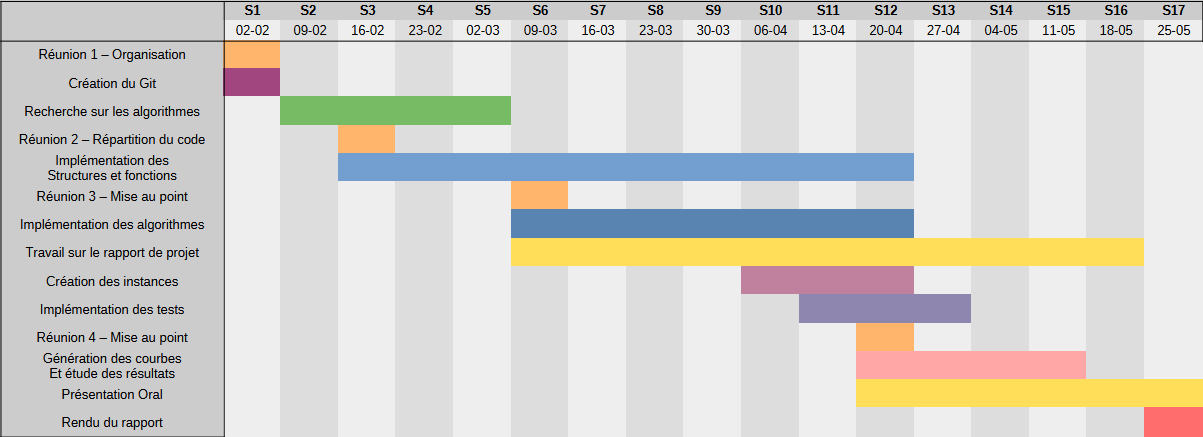
\includegraphics[width=1\textwidth]{Gantt2.png}
    \caption{Diagramme de Gantt}
    \label{fig:example}
\end{figure}

Le projet a débuté par une réunion d'organisation (semaine 1), au cours de laquelle les objectifs ont été clarifiés, les outils de travail définis, et une répartition préliminaire des rôles a été effectuée. Lors de cette réunion, le dépôt Github a été créé pour permettre un travail collaboratif et un suivi des versions du code source.\\

Nous avons ensuite entamé une période de recherche sur les algorithmes. En effet, ce projet relevant quasi-intégralement de l'algorithmique, il était essentiel que tous les membres se renseignent et étudient en profondeur tous les algorithmes qui vont être implémentés. Cette étape a donc permis à tous les membres d'être à l'aise avec le fonctionnement des différents algorithmes avant de les implémenter. Elle a également permis d'identifier les approches les plus adaptées aux besoins du projet, et de poser les bases pour la phase de développement.\\

Nous nous sommes à nouveau retrouvé semaine 3 pour discuter de l'avancement de la recherche et de la mise en place des algorithmes. Nous avons choisi notre langage de programmation, C\#, et nous sommes mis d'accord sur la structure pour commencer à développer les premières classes.\\

Nous nous sommes répartis les algorithmes à implémenter, et chacun a commencé à travailler sur son propre algorithme. Nous avons également attribué la tâche de la création des instances à un membre de l'équipe ainsi que celle de la création des tests unitaires. En parallèle, nous avons commencé à travailler sur le rapport, chacun sur sa partie. Lorsque tout était correctement implémenté, nous avons pu lancer les séries de calculs sur les différents algorithmes et ainsi produire les résultats et les courbes de performance dont font l'objet ce TER.

\subsection*{Travail collaboratif avec Git}

Étant quatre à travailler sur ce projet, nous avons utilisé \textbf{Git} comme système de gestion de versions pour organiser notre développement de manière collaborative et efficace. Git nous a permis de partager le code en temps réel, de suivre l’évolution de chaque fonctionnalité, et de travailler en parallèle sans conflits majeurs.

Chaque membre du groupe a pu développer des parties spécifiques du projet dans des branches séparées, avant de les fusionner dans la branche principale une fois validées. Cela a facilité le développement et réduit les risques d’écrasement de code. Grâce à l’historique de Git, nous avons également pu revenir facilement à des versions antérieures si nécessaire.

L'utilisation de Git nous a donc permis de structurer le projet comme une véritable équipe de développement logiciel, en mettant en pratique des outils largement utilisés dans l'industrie, et en rendant notre travail plus rigoureux et traçable.

Le dépôt du projet est accessible à l’adresse suivante :  
\url{https://github.com/Wronskode/Flot-maximum}



\subsection{Présentation des classes}

Dans cette section, nous présentons les différentes classes développées dans le cadre de ce projet, ainsi que leur rôle et leurs interactions.

Les classes principales que nous avons implémentées sont les suivantes :

\begin{itemize}
    \item \textcolor{violet}{Vertex}
    \item \textcolor{violet}{Graph}
    \item \textcolor{violet}{FlowNetwork}
    \item \textcolor{violet}{FileFlowNetwork}
    \item \textcolor{violet}{RandomFlowNetwork}
    \item \textcolor{violet}{Flow}
    \item \textcolor{violet}{PL}
    \item \textcolor{violet}{Curve}
    \item \textcolor{violet}{Program}
\end{itemize}

Nous détaillons maintenant chacune de ces classes en exposant leur conception, leurs fonctionnalités principales, ainsi que leur rôle dans le fonctionnement global du projet.

\subsubsection{Vertex}

La classe \textcolor{violet}{Vertex} représente un sommet dans un graphe. Chaque sommet est identifié par un nom ou une étiquette, généralement une chaîne de caractères. Cette classe permet d'identifier et de manipuler les nœuds du graphe. Deux sommets sont considérés comme égaux s'ils portent le même nom, ce qui autorise leur utilisation comme clés dans des dictionnaires, notamment pour stocker les arêtes, les capacités ou les flots.

\subsubsection{Graph}

La classe \textcolor{violet}{Graph} représente un graphe orienté pondéré, outils de base pour tous nos algorithmes. En effet la classe \textcolor{violet}{FlowNetwork}, qui représente un réseau le réseau de flot qu'on va utiliser, hérite de la classe \textcolor{violet}{Graph}. Un objet de \textcolor{violet}{Graph} est défini par deux dictionnaires : \textcolor{blue!60}{AdjVertices}, qui associe chaque sommet à l'ensemble de ses successeurs, et \textcolor{blue!60}{Edges}, qui stocke les arêtes du graphe avec leur capacité sous forme de couple de sommets.
Quelques fonctions de bases sont codées, comme par exemple \textcolor{green!60!black}{NeighborsLeft} où \textcolor{green!60!black}{NeighborsRight}, qui retournent respectivement les voisins entrants et sortants d'un sommet donné, une fonction \textcolor{green!60!black}{Clone} qui clone le graphe et d'autres fonctionnalités classiques.

\subsubsection{FlowNetwork}

La classe \textcolor{violet}{FlowNetwork} est au cœur de la bibliothèque de calcul de flot maximal. Elle étend la structure de base \textcolor{violet}{Graph} en introduisant plusieurs notions fondamentales. C'est depuis cette classe que l'on va gérer tout les algorithmes de calcul de flot maximum qui consituent le coeur de ce projet. Nous nous proposons donc naturellement de détailler cette classe, qui est la plus importante.\\

En plus de l'héritage de la classe \textcolor{violet}{Graph}, la classe \textcolor{violet}{FlowNetwork} introduit les attributs \textcolor{blue!60}{Source} et \textcolor{blue!60}{Puits}, qui représentent respectivement le sommet source et le sommet puits du réseau. Ces attributs sont essentiels pour les algorithmes de flot maximal, car ils définissent les points d'entrée et de sortie du réseau.\\

Cette classe concentrant tout les algorithmes de calcul sur un réseau de flot, elle contient évidement tout les algorithmes de de calcul de flot maximum que nous avons implémentés. Nous en redonnons ici une liste non exhaustive :
\begin{itemize}
	\item \textcolor{green!60!black}{FordFulkerson}
	\item \textcolor{green!60!black}{EdmondsKarp}
	\item \textcolor{green!60!black}{Dinic}
	\item \textcolor{green!60!black}{PushRelabel}
\end{itemize}
La résolution via la programmation linéaire fait l'objet d'une classe séparée, \textcolor{violet}{PL}, car cette méthode ne constitue pas réellement en elle même un algorithmes sur les réseaux de flot.\\

Plusieurs fontions essentielles aux fonctionnement de ces algorithmes où à d'autres taches telles que la constructions d'instances on également été implémentées. En voici les plus importantes :
\begin{itemize}
	\item \textcolor{green!60!black}{DFS\_GetPathInLevelGraph} : implémente une recherche en profondeur (DFS) pour trouver un chemin augmentant dans un graphe résiduel (typiquement dans l'algorithme de FordFulkerson ou de Dinic).
	\item \textcolor{green!60!black}{BFS\_GetLevels} : utilise une recherche en largeur (BFS) pour attribuer à chaque sommet son niveau (distance minimale en nombre d’arêtes depuis la source) dans un graphe.
	\item \textcolor{green!60!black}{GetResidualGraph} : permet de récupérer le graphe résiduel du réseau de flot.
	\item \textcolor{green!60!black}{GetMaxFlow} : permet de récupérer la valeur du flot maximum. L'interêt et les propriétés d'un tel graphes sont détaillés dans la section sur les algorithmes de flot maximum.
	\item \textcolor{green!60!black}{IsConnected} : cette méthode n'est pas utilisée dans les algorithmes de flot maximum, mais elle a été très utile lors de la création des instances. En effet, elle permet de vérifier plusieurs propriétés sur le graphe qui sont essentielles pour s'assurer que le graphe est \og{}bien formé\fg{}. Comme détaillé dans la partie sur les instances, elle vérifie que tout sommet est accessible depuis la source et que tout sommet admet un chemin jusqu'au puits. Elle décide donc si un graphe est gardé comme instance ou jeté.
	\item \textcolor{green!60!black}{CreateGraphFile} : permet de créer un fichier texte contenant la représentation du graphe. Cette méthode est utilisée lors de la création des instances, afin de pouvoir les sauvegarder et les réutiliser plus tard.
\end{itemize}
Pour plus de precisions sur le fonctionnement des méthodes relatives aux algorithmes de flot maximum, nous vous renvoyons à la \hyperref[sec:algos]{\textcolor{black}{section sur les algorithmes de flot maximum.}}

\subsubsection{FileFlowNetwork}

La classe \textcolor{violet}{FileFlowNetwork} a pour rôle de générer dynamiquement un réseau de flot (\textcolor{violet}{FlowNetwork}) à partir d’un fichier texte structuré. Elle lit dans ce fichier les informations nécessaires à la construction du graphe : l'identifiant du sommet source, celui du puits, puis une liste d’arêtes définies par deux sommets et une capacité. Le fichier est lu ligne par ligne, chaque sommet étant instancié sous forme d’objet \textcolor{violet}{Vertex}, et les arêtes ajoutées avec leur poids dans un objet \textcolor{violet}{Graph}. À la fin de la lecture, la méthode \textcolor{green!60!black}{Generate} de la classe construit et retourne une instance de \textcolor{violet}{FlowNetwork} contenant la topologie complète du graphe, prête à être utilisée dans les algorithmes de flot maximum.

\subsubsection{RandomFlowNetwork}
La classe \textcolor{violet}{RandomFlowNetwork} est responsable de la génération aléatoire de graphes orientés, qui sont ensuite utilisés comme instances pour les algorithmes de flot maximum. Elle crée un graphe orienté en ajoutant des sommets et des arêtes de manière aléatoire, tout en respectant une densité spécifiée. La classe permet également de définir une source et un puits, ainsi que d'assigner des capacités aux arêtes. Sa méthode \textcolor{green!60!black}{Generate} retourne un objet \textcolor{violet}{FlowNetwork} représentant le réseau de flot. La methode de génération de graphes aléatoires est détaillée dans la \hyperref[sec:creer_instances]{\textcolor{black}{section sur la création des instances}}.

\subsubsection{Flow}

La classe \textcolor{violet}{Flow} est utilisée pour représenter un flot, soit la fonction $f : V^2 \to \mathbb{R}$ que nous étudions. Cette classe permet de stocker et de manipuler les flots calculés par les différents algorithmes de flot maximum.

\subsubsection{PL}

La classe \textcolor{violet}{PL} (Programmation Linéaire) a pour rôle de modéliser le problème du calcul du flot maximum sur un graphe donné sous la forme d’un système linéaire, puis de le résoudre à l’aide de solveurs spécialisés tels que Google OR-Tools ou Gurobi. Elle construit un modèle dans lequel chaque variable représente le flot sur une arête, les contraintes traduisent les capacités maximales des arêtes et les lois de conservation du flot en chaque sommet intermédiaire (autres que la source et le puits), et la fonction objectif vise à maximiser le flot total sortant de la source. La méthode \textcolor{green!60!black}{SolveWithOrTools} implémente cette logique avec OR-Tools, tandis que \textcolor{green!60!black}{SolveWithGurobi} l’implémente via l’API Gurobi. Une méthode \textcolor{green!60!black}{AfficherSysteme} est également disponible pour visualiser les variables, les contraintes et la fonction objectif du système linéaire généré. Pour plus de détails nous vous renvoyons à la \hyperref[sec:pl]{\textcolor{black}{section sur la programmation linéaire}}.

\subsubsection{Curve}

La classe \textcolor{violet}{Curve} est chargée de mesurer les performances temporelles de différents algorithmes de calcul du flot maximum sur un ensemble d’instances de graphes, puis de générer automatiquement des courbes de benchmark. Pour une densité donnée, la méthode \textcolor{green!60!black}{CreateCurves} parcourt tous les fichiers de graphes correspondants dans un dossier, instancie le réseau de flot associé, et exécute chaque algorithme de calcul fourni tout en mesurant le temps d’exécution. Ces temps sont ensuite agrégés en fonction du nombre de sommets du graphe, permettant ainsi de tracer des courbes de performance (temps en fonction du nombre de sommets) pour chaque méthode. La bibliothèque ScottPlot est utilisée pour la génération des graphiques, qui sont ensuite enregistrés au format PNG. Cette classe permet donc de produire les courbes qui nous permettent de visualiser la complexité pratique des algorithmes de flot maximum en fonction de la taille du graphe.

\subsubsection{Program}

Cette \textcolor{violet}{Program} classe principale constitue le point d'entrée du programme. C’est depuis ce fichier que l’on appelle les différentes classes développées dans le projet pour effectuer les diverses actions nécessaires : génération des instances aléatoires, résolution du problème de flot maximum à l’aide de plusieurs algorithmes, et création des courbes de performances. Elle orchestre ainsi l’ensemble du processus expérimental, de la construction des graphes jusqu’à l’analyse des résultats.

\subsection{Langage et classes}

Pour ce projet de TER, nous avons décidé d’utiliser le langage C\#. Ce choix nous a semblé pertinent car C\# est un langage moderne, orienté objet, avec une syntaxe claire et bien structurée. Cela nous a permis de développer notre code de manière propre et organisée, ce qui est important quand on travaille sur plusieurs algorithmes comme ceux de flot.

Nous avons utilisé l’environnement de développement Rider (JetBrains), qui offre de nombreux outils utiles comme l’autocomplétion, la navigation dans le code, le refactoring ou encore un bon débogueur \cite{jetbrains_rider}. Ces fonctionnalités nous ont vraiment facilité le développement et nous ont permis de rester concentrés sur l’essentiel : l’implémentation des algorithmes et l’analyse de leurs performances.

Plutôt que d’utiliser une bibliothèque externe, nous avons choisi d’implémenter nous-mêmes les structures de graphes nécessaires (nœuds, arêtes, flot, etc.). Cette approche nous a permis de mieux comprendre le fonctionnement interne des algorithmes et d’adapter notre représentation à leurs besoins spécifiques.

Même si C\# n’est pas le langage le plus utilisé dans les publications en algorithmique (où C++ ou Python sont plus populaires), il reste suffisamment performant pour notre projet. De plus, il offre un bon compromis entre lisibilité, facilité de prise en main, et performances, ce qui en fait un choix raisonnable pour un projet de recherche appliquée encadré.
\subsection{Tests}
Tout au long du projet, nous avons mis en place des tests unitaires pour vérifier le bon fonctionnement de nos algorithmes et de nos classes. Ces tests ont été réalisés à l'aide du framework de test intégré à Rider, qui nous a permis d'écrire des tests clairs et faciles à maintenir.

Nous vérifions notamment que les algorithmes de flot maximum renvoyaient bien le flot maximum attendu pour des instances connues, et que les graphes générés étaient bien formés (connectés, avec une source et un puits valides). Ces tests nous ont permis de garantir la robustesse de notre code et de détecter rapidement d'éventuelles régressions lors des modifications. Nous testons nos algorithmes sur des centaines, voir des milliers d'instances aléatoirement générées, ce qui nous permet de nous assurer que les algorithmes fonctionnent correctement dans une grande variété de cas.
\section{Méthodologie Expérimentale}


\section{Courbes, Résultats et Discussion}
Après avoir conçu et implémenté l’ensemble des algorithmes de flot maximal, ainsi que l’infrastructure de génération d’instances de graphes, nous présentons ici la mise en œuvre expérimentale et l’analyse comparative des performances des différentes approches. L'objectif du TER était entre autres de comparer les algorithmes de flot maximum et pour cela nous avons généré différentes courbres de performance. Nous avons choisi de représenter les performances en fonction du nombre de sommets du graphe, car c'est un indicateur pertinent de la complexité des algorithmes.\\

\subsection{Avec $n_{max} = 100$}
Afin de pouvoir commencer notre analyse nous présentons d'abord ce premier graphique :

\begin{figure}[h]
    \centering
    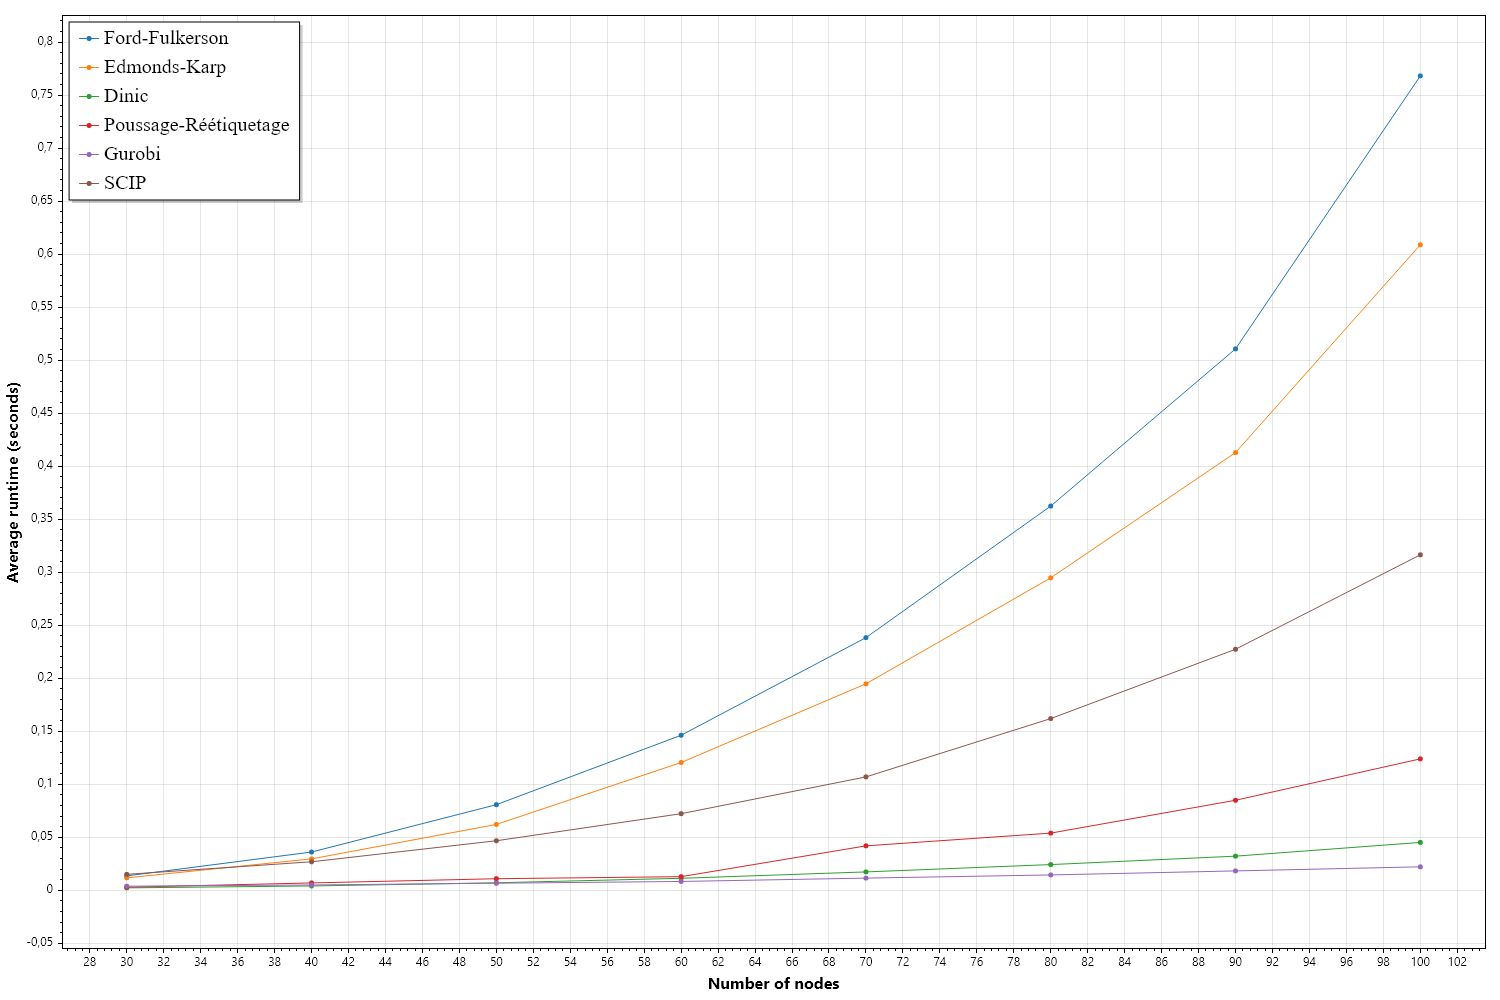
\includegraphics[width=1\textwidth]{courbes/benchmark_global_average_100.png}
    \caption{Temps de convergence en fonction du nombre de sommets avec $n_{max} = 100$}
    \label{fig:example}
\end{figure}

Cette première figure représente les performances de tous les algorithmes de flot maximum que nous avons implémentés. pour chaque point du graphe, nous avons fait la moyenne sur toutes les instances de même taille. Il y a ainsi 8 tailles différentes, de 30 à 200, on a donc $n \in \left\{30, 40, 50, 60, 70, 80, 90, 100, 120, 150, 200\right\}$, et pour chaque taille nous avons 4 densités différentes avec $d \in \left\{0.3, 0.5, 0.7, 0.9\right\}$ nous avons enfin 5 instances par densité. Chaque point est donc la moyenne de 20 instances.\\

Pour cette première figure nous ne dépassons pas $n = 100$ car au delà de cette taille, les algorithmes de Ford-Fulkerson et d'Edmonds-Karp deviennent trop lents prendraient trop de temps pour converger. Aussi leurs comparaisons avec les autres algorithmes ne seraient pas pertinentes. Les autres courbes se confondraient en bas du graphique pendant que Ford-Fulkerson et Edmonds-Karp exploseraient. Nous etudierons donc les algorithmes de flot maximum sur des graphes de taille supérieure séparement.\\

Afin de commenter ces courbes, nous rappelons d'abord la complexité théorique de chaque algorithme :

\begin{table}[H]
	\centering
	\begin{tabular}{|c|c|c|}
		\hline
		Algorithme & Complexité & Complexité en fonction de $n = |V|$ \\
		\hline
		Ford-Fulkerson & $O(|E|f^\star)$ &$O(n^2 f^\star)$\\
		Edmonds-Karp & $O(|V||E|^2)$ &$O(n^5)$\\
		Dinic & $O(|V|^2|E|)$& $O(n^4)$\\
		Poussage-Réétiquetage & $O(|V|^2|E|)$&$O(n^4)$ \\
		\hline
	\end{tabular}
	\caption{Récapitulatif des algorithmes de flot maximum}
\end{table}

Nous pouvons constater le graphe ne présente aucune irrégularité, tester sur autant d'instances permet en effet d'harmoniser et de trouver un résultat proche de ce que l'on attend en étudiant la complexité théorique.\\

Les premières courbes obtenues confirment clairement les écarts de complexité algorithmique entre les différentes méthodes étudiées. On observe que chaque algorithme occupe une position cohérente sur la courbe, en accord avec sa complexité théorique. Les approches naïves, telles que Ford-Fulkerson ou Edmonds-Karp, présentent une croissance rapide du temps d'exécution à mesure que la taille des graphes augmente, ce qui reflète leur complexité plus élevée.\\

À l'inverse, des algorithmes plus avancés comme Dinic ou le Poussage-Réétiquetage, reconnus pour leur meilleure complexité théorique, se distinguent par une meilleure scalabilité. Leur temps d'exécution croît de manière bien plus modérée, ce qui les rend plus adaptés aux grands graphes.\\

Concernant les solveurs de type PLNE, tels que Gurobi et SCIP, une différence de performance nette se dégage. SCIP s’avère significativement plus lent : il est environ deux fois plus long que l’algorithme de Poussage-Réétiquetage et jusqu’à dix fois plus lent que Dinic. À l’inverse, Gurobi offre des performances remarquables, surpassant l’ensemble des autres méthodes, y compris les algorithmes les plus puissants. Cela s’explique notamment par la sophistication de son infrastructure logicielle : Gurobi repose sur un moteur d’optimisation hautement performant, mais en grande partie opaque, fonctionnant comme une \og{}boîte noire\fg{}. À l’opposé, SCIP semble adopter une approche plus basique, plus proche d’une résolution manuelle d’un système linéaire, sans optimisation poussée des données ni techniques avancées de réduction du problème. De plus, il convient de noter que le temps d’exécution des solveurs de type PLNE inclut non seulement la résolution du programme linéaire, mais aussi la phase de modélisation du graphe en tant que programme linéaire. Cette conversion reste cependant peu coûteuse, comme en témoignent les excellentes performances de Gurobi. En effet, si cette phase de modélisation prenait le pas sur la résolution elle-même, Gurobi et SCIP présenteraient des temps d’exécution similaires à mesure que la taille des instances augmente. Ce n'est cependant pas le cas, on peut donc bien dire que les resultats obtenus témoignent bien de la complexité de résolution du système.\\

On peut constater que les résultats sont en parfaite adéquation avec la littérature algorithmique, validant ainsi notre implémentation et notre protocole expérimental.


\subsection{Avec $n_{max} = 500$}

\begin{figure}[H]
    \centering
    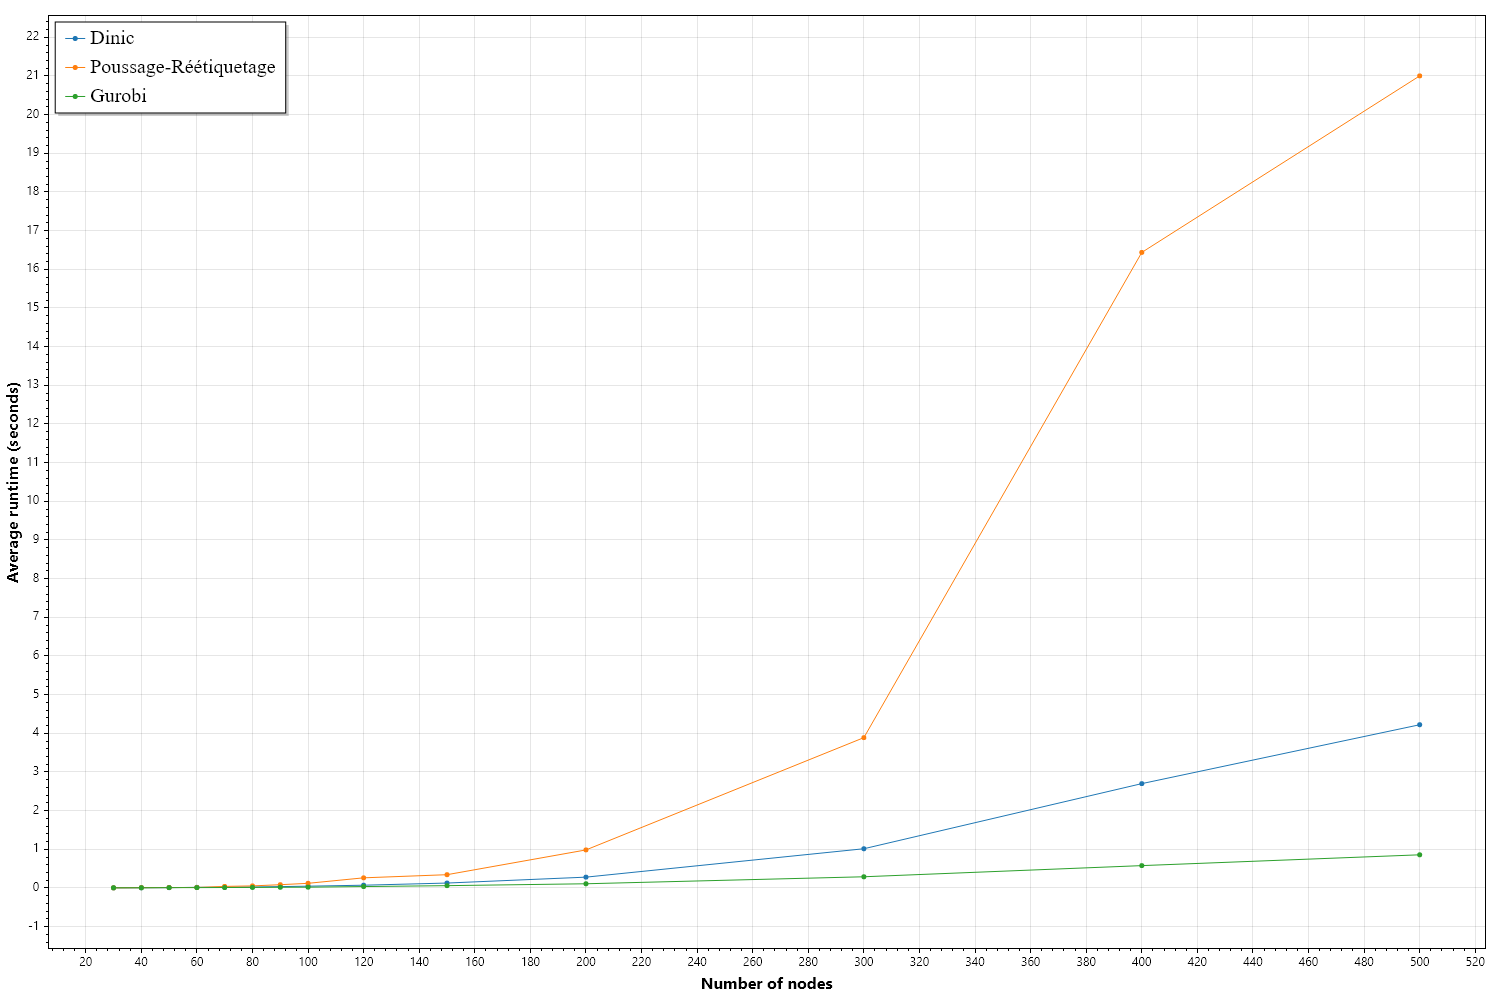
\includegraphics[width=1\textwidth]{courbes/benchmark_global_average_500.png}
    \caption{Temps de convergence en fonction du nombre de sommets avec $n_{max} = 500$}
    \label{fig:example}
\end{figure}

Sur cette seconde courbe (jusqu’à 500 nœuds), on observe de manière encore plus marquée la divergence de performance entre les trois algorithmes comparés :\\

Poussage-Réétiquetage devient très coûteux en temps à partir d’environ 300 sommets. Son temps d'exécution explose, atteignant plus de 20 secondes pour 500 nœuds. Cela reflète les limites pratiques de cet algorithme sur des instances plus grandes, malgré sa bonne complexité théorique. Dinic conserve une progression régulière, avec un temps d'exécution qui augmente de manière maîtrisée. Il s'agit donc d’une méthode performante et stable sur des graphes de taille moyenne à grande. Gurobi, encore une fois, se démarque nettement : son temps d’exécution reste très faible, quasiment constant jusqu’à 500 sommets. Cela démontre la puissance de son moteur d’optimisation, capable de traiter efficacement de grands graphes en très peu de temps.

\subsection{Avec $n_{max} = 500$}

\begin{figure}[H]
    \centering
    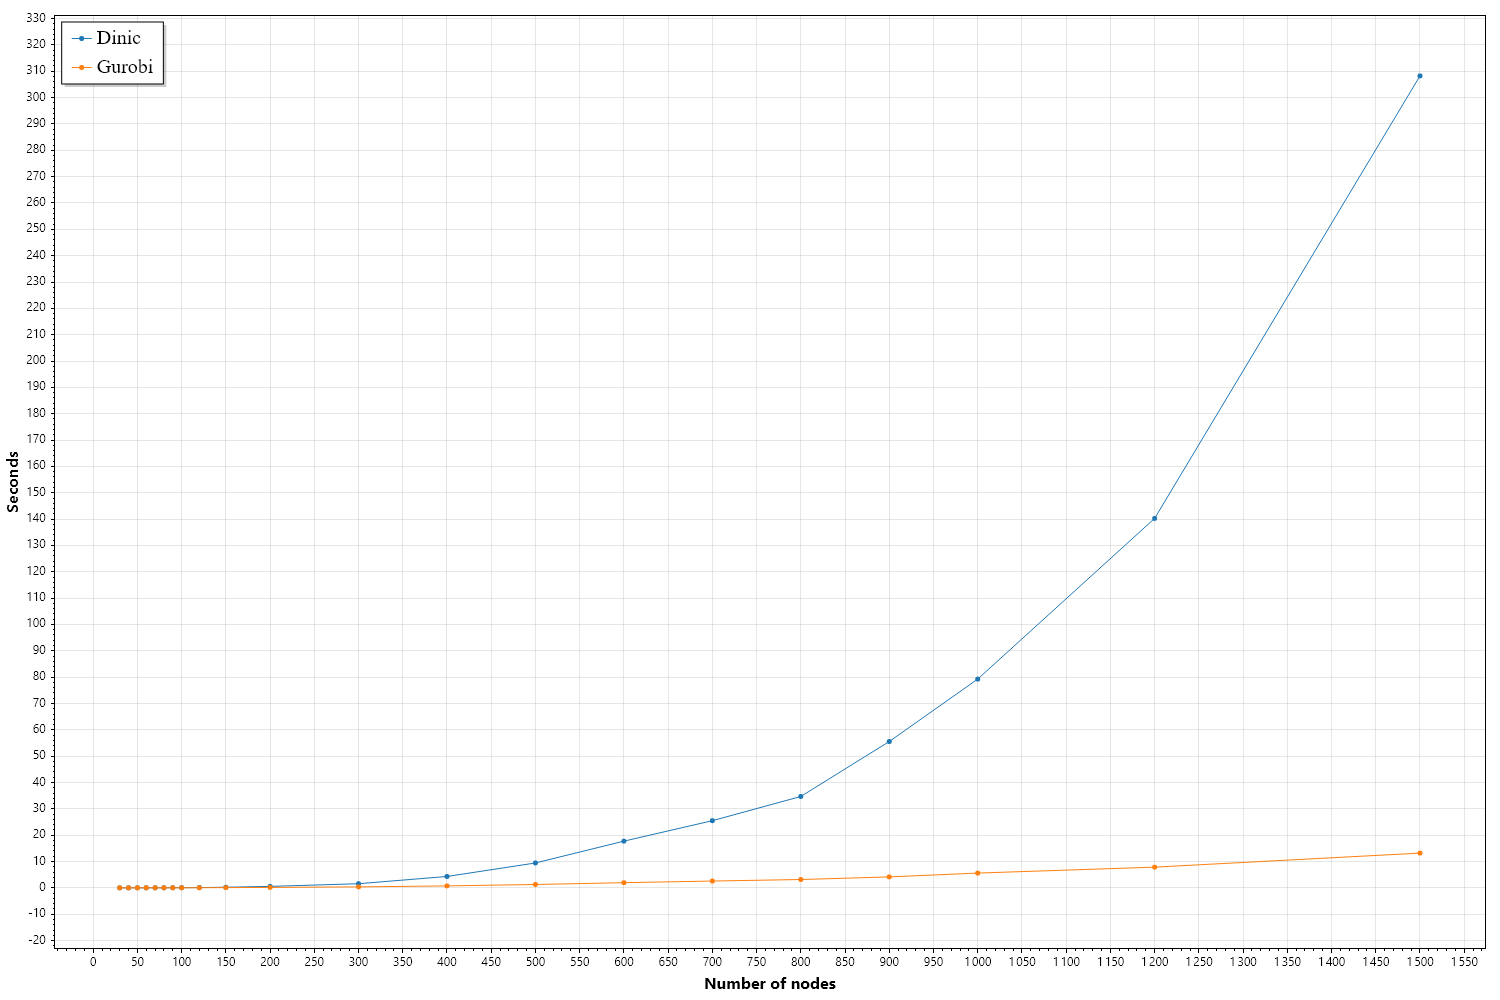
\includegraphics[width=1\textwidth]{courbes/benchmark0,7_2000.png}
    \caption{Temps de convergence en fonction du nombre de sommets avec $n_{max} = 2000$}
    \label{fig:example}
\end{figure}

Quelques tests ont également été effectués sur des instances de très grande taille, comportant jusqu’à 2000 sommets. On aura pu comparer uniquement l'algorithmes de Dinic et le solver Gurobi, car les autres algorithmes deviennent trop lents pour converger sur des instances de cette taille en temps raisonnable. Bien que l’algorithme de Dinic, reconnu pour son efficacité, parvienne à résoudre ces instances, il nécessite tout de même plusieurs minutes d’exécution. À l’inverse, Gurobi continue de se distinguer par sa rapidité, ne mettant que quelques secondes pour atteindre une solution, même sur ces très grandes tailles.\\

\subsection{Densités spécificiques}

\begin{figure}[H]
    \centering
    \begin{subfigure}[b]{0.45\textwidth}
        \centering
        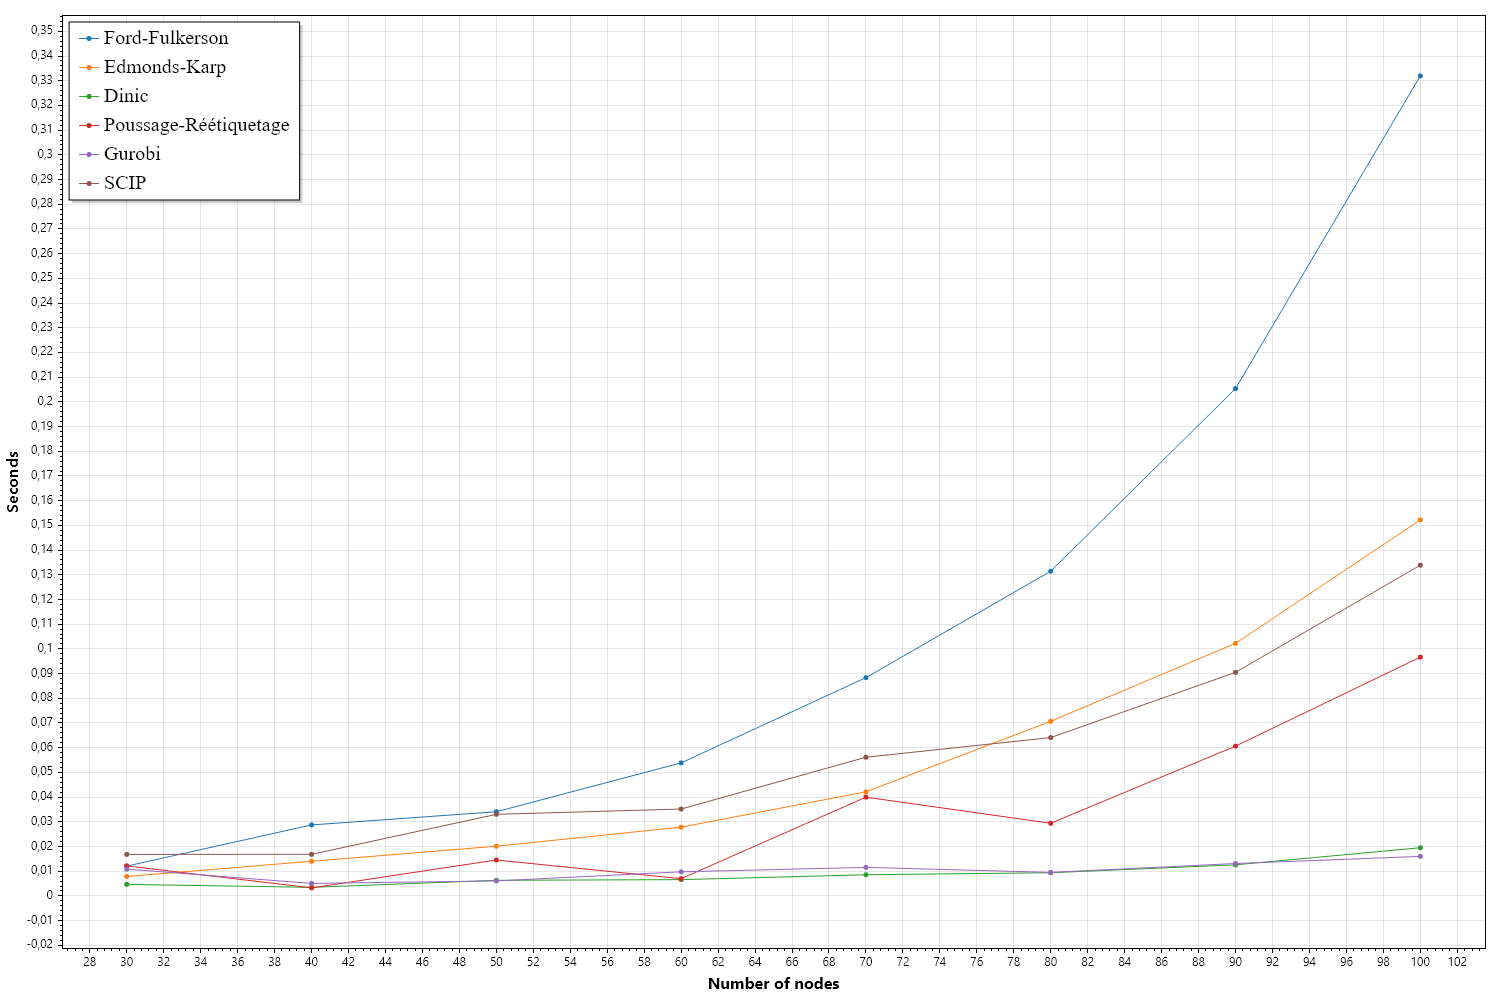
\includegraphics[width=\textwidth]{courbes/benchmark0,3_100.png}
        \caption{Courbes densité $0{,}3$}
        \label{fig:image1}
    \end{subfigure}
    \hfill
    \begin{subfigure}[b]{0.45\textwidth}
        \centering
        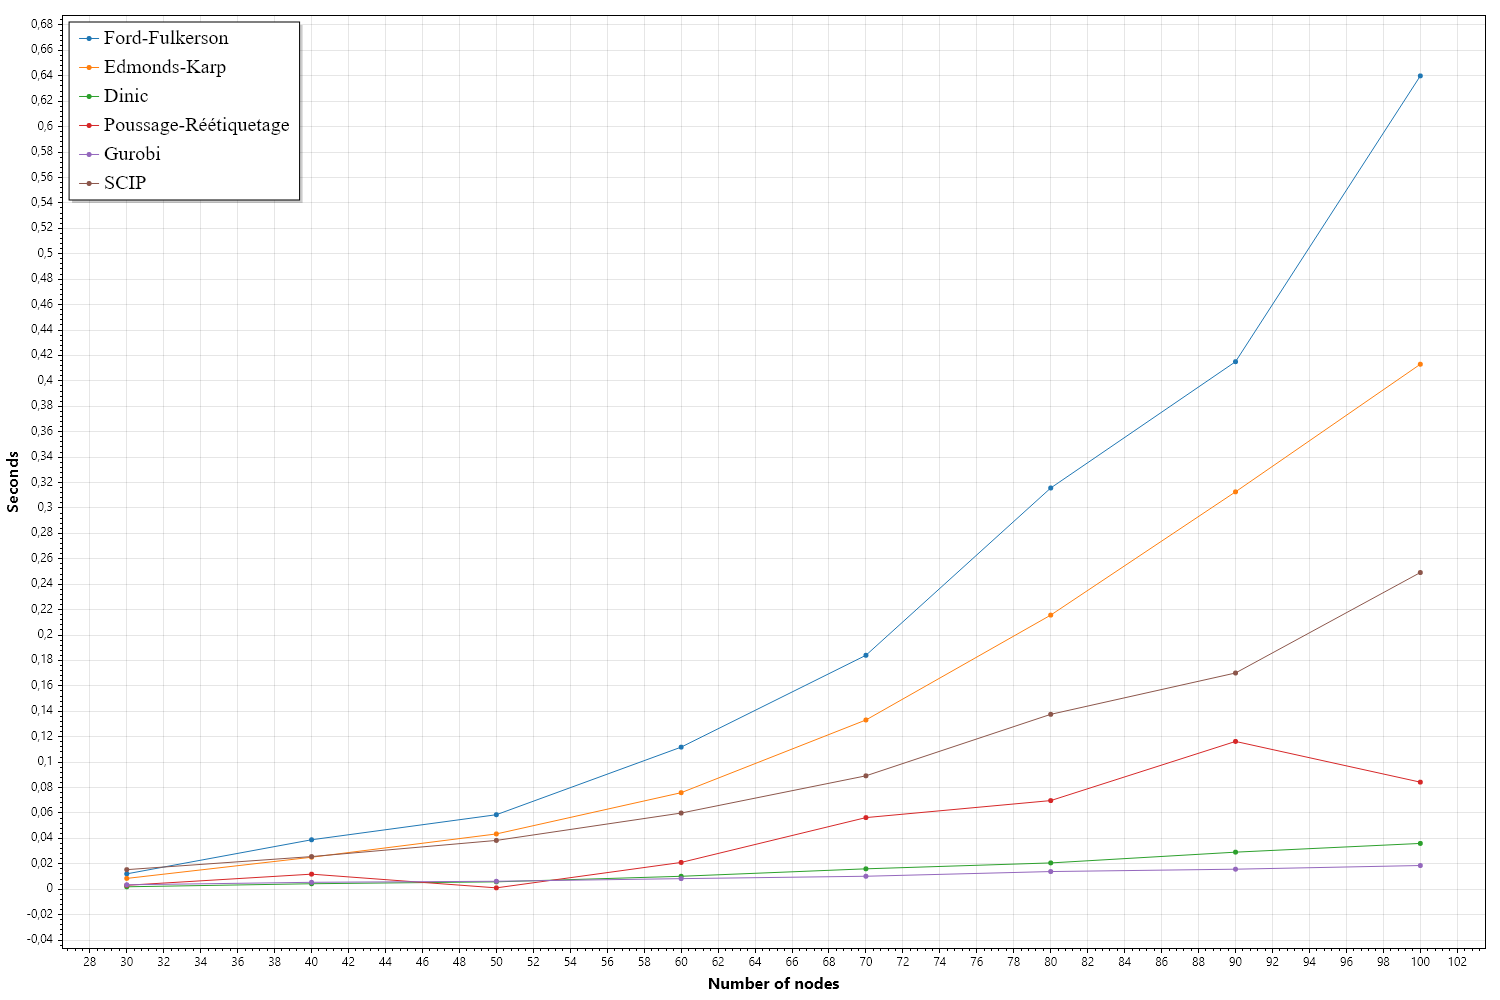
\includegraphics[width=\textwidth]{courbes/benchmark0,5_100.png}
        \caption{Courbes densité $0{,}5$}
        \label{fig:image2}
    \end{subfigure}
    \vskip\baselineskip
    \begin{subfigure}[b]{0.45\textwidth}
        \centering
        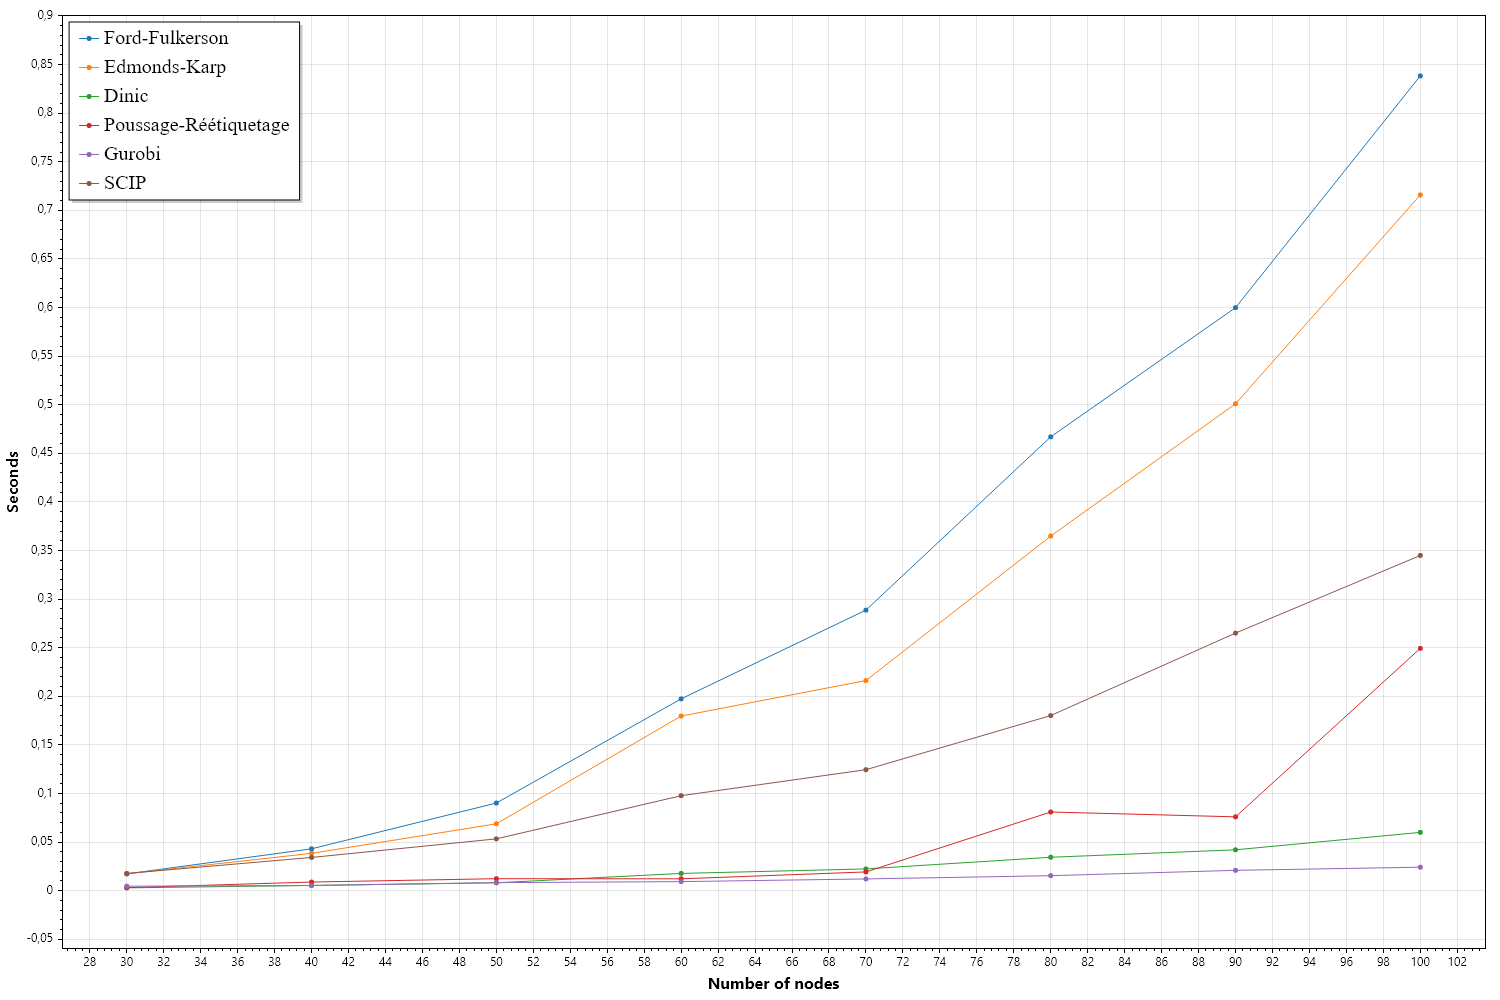
\includegraphics[width=\textwidth]{courbes/benchmark0,7_100.png}
        \caption{Courbes densité $0{,}7$}
        \label{fig:image3}
    \end{subfigure}
    \hfill
    \begin{subfigure}[b]{0.45\textwidth}
        \centering
        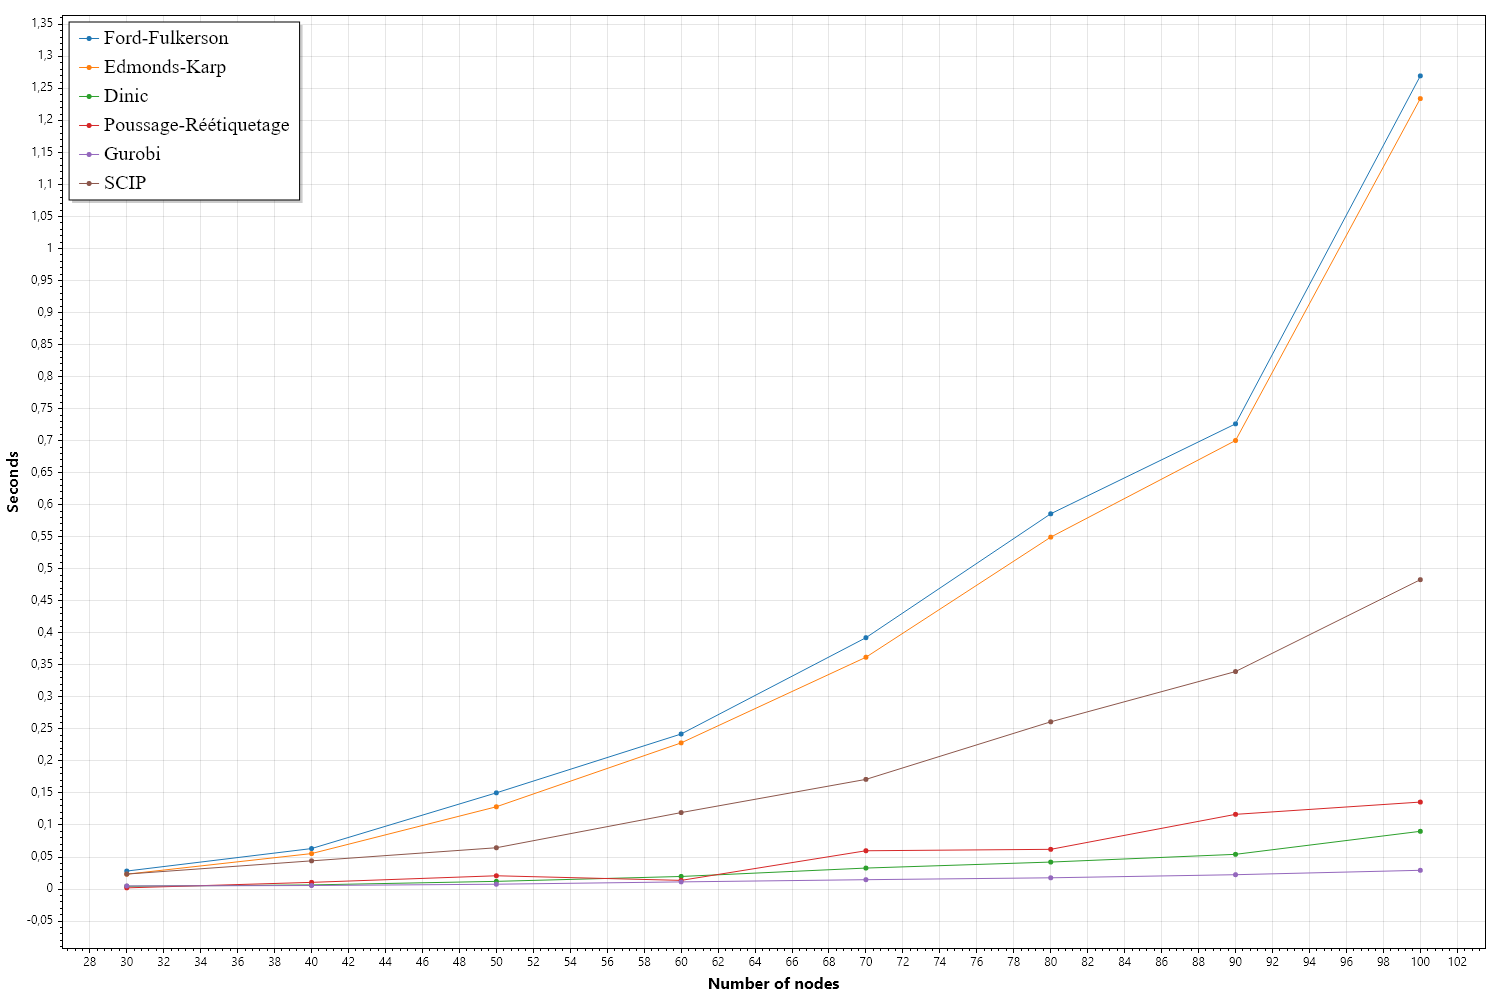
\includegraphics[width=\textwidth]{courbes/benchmark0,9_100.png}
        \caption{Courbes densité $0{,}9$}
        \label{fig:image4}
    \end{subfigure}
    \caption{Comparaisons pour les différentes densités}
    \label{fig:group}
\end{figure}

Les expérimentations ont été menées sur des graphes de densités variées, allant de très clairsemés à fortement connectés. Un constat remarquable est que, malgré ces variations structurelles, l’ordre de performance entre les algorithmes reste strictement inchangé. Autrement dit, quel que soit le nombre d’arêtes dans les graphes, les algorithmes les plus rapides conservent leur avance, tandis que les plus lents restent en queue de classement.\\

Ce phénomène témoigne d’une certaine robustesse des méthodes évaluées : leur comportement asymptotique est gouverné principalement par leur complexité algorithmique propre, et non par des variations contextuelles comme la densité du graphe. Cela renforce la pertinence de cette comparaison expérimentale, en montrant que les écarts de performance sont structurels et non accidentels.

\subsection{Observation générale}

Parmi les différents algorithmes évalués pour résoudre le problème de flot maximum, les résultats expérimentaux montrent des écarts de performance marqués, directement liés à leurs principes algorithmiques. Ford-Fulkerson est de loin le plus lent : son approche naïve par chemins augmentants sans stratégie d’optimisation le rend peu adapté aux grandes instances. Edmonds-Karp améliore légèrement la situation grâce à l’utilisation de chemins les plus courts, mais reste limité par une complexité en O(VE²). Vient ensuite SCIP, un solveur généraliste de programmation linéaire, qui reste moins performant qu’on ne pourrait l’attendre, probablement en raison d’un manque d’optimisation spécifique pour ce type de problème.\\

En revanche, l’algorithme de poussage-réétiquetage se révèle bien plus efficace : en se basant sur des opérations locales et une gestion intelligente des hauteurs, il limite considérablement le nombre de recalculs. Dinic fait encore mieux grâce à sa stratégie basée sur les niveaux et les envois de flots par blocs, ce qui le rend particulièrement performant, même sur de grandes tailles. Il s'agit du seul algorithme de résolution implémenté (hors programmation linéaire) capable de s'exécuter en un temps raisonnable sur des instances de très grande taille. Enfin, Gurobi, grâce à ses techniques d’optimisation industrielles et son efficacité dans la résolution des modèles linéaires, se démarque comme le plus rapide dans ces tests.




\section{Revue de la littérature avancée}
Les algorithmes classiques de flot maximal comme ceux de Ford-Fulkerson, Dinic ou Poussage-Réétiquetage ont longtemps constitué l’état de l’art pratique et théorique. Cependant, des avancées majeures ont été réalisées dans la dernière décennie en algorithmique théorique, avec l’apparition d’algorithmes extrêmement rapides reposant sur des outils sophistiqués d’optimisation, d’algèbre linéaire et de structures de graphes dynamiques.

Ces algorithmes atteignent pour la première fois une complexité proche ou quasi-linéaire, dans certains cas, en combinant des approches structurelles (arborescences, décompositions récursives), des techniques de descente de potentiel (interior point methods), ou encore des méthodes de résolution de systèmes linéaires dans les graphes.

\subsection{Algorithme BLNPSSSW (2020)}
L’algorithme proposé par \textbf{Bernstein, Liu, Nanongkai, Probst Gutenberg, Sidford, Spinrad, Sun et Wang} en 2020 marque une percée dans l’optimisation du flot maximal\cite{chen2022maximumflowminimumcostflow}. Il atteint une complexité de :
\[
\tilde{\mathcal{O}}((E+ V^{3/2} - \varepsilon)log U)
\]
pour un certain $\varepsilon > 0$, soit une amélioration significative par rapport aux bornes précédentes.

Leur approche repose sur la réduction du problème de flot maximum à des problèmes de circulation avec capacités, qui sont ensuite résolus par une combinaison de techniques :
\begin{itemize}
    \item résolution de systèmes linéaires dans des matrices de Laplace,
    \item descente de potentiel (interior-point methods),
    \item préconditionnement et sparsification de graphes.
\end{itemize}
Ici \[\tilde{\mathcal{O}}\] indique une complexité asymptotique qui ignore certains facteurs logarithmiques. Plus précisément, la définition exacte est la suivante :
\begin{definition} Soit $f: \mathbb{N} \to \mathbb{R}^+$ et $g: \mathbb{N} \to \mathbb{R}^+$ deux fonctions. Si $g$ est polynomiale en $n$, on dit que
	$f(n) = \tilde{\mathcal{O}}(g(n))$ si  $f(n) = \mathcal{O}(g(n) \log^k n)$ pour un $k \in \mathbb{N}$.
\end{definition}
C’est l’un des premiers résultats à montrer qu’on pouvait battre rigoureusement la barrière des $\mathcal{O}(m \sqrt{n})$ pour les graphes généraux.
\subsection{Algorithme de Gao-Liu-Peng (2021)}
Proposé par \textbf{Gao, Liu et Peng}, cet algorithme repose sur l’observation que le problème de flot maximal peut être résolu à l’aide de méthodes de préconditionnement et de raccourcissement de chemins dans les graphes\cite{gao2021fullydynamicelectricalflows}. En appliquant une stratégie d’approximation contrôlée, les auteurs parviennent à une complexité :
\[
\tilde{\mathcal{O}}\left(E^{\frac{3}{2} - \frac{1}{32\delta}} \log U\right)
\]
avec des garanties sur l’erreur relative du flot obtenu.

Leur méthode repose notamment sur des techniques hybrides entre les algorithmes de flot bloquant et la résolution approchée de systèmes linéaires associés aux graphes.

\subsection{Algorithme de Chen, Kyng, Liu, Peng, Gutenberg, Sachdeva (2022)}
Ce collectif d’auteurs a contribué à généraliser et raffiner les algorithmes de flot maximal en s’appuyant sur des outils puissants de l’algèbre linéaire numérique, notamment les solveurs Laplaciens.

L’approche consiste à ramener le flot maximum à un problème de minimisation de potentiel dans un graphe résiduel, résolu par une succession de systèmes linéaires approchés\cite{chen2022maximumflowminimumcostflow}. Les résultats atteignent des complexités du type :
\[
\mathcal{O}\left(E^{1 + o(1)} \log U\right)
\]
dans certains cas, avec de très bonnes constantes pratiques.

Leur travail fait partie d’une série d’efforts visant à transposer les méthodes numériques continues (optimisation convexe, gradients, projections) à des problèmes discrets de flot.

\subsection{Conclusion}
Ces algorithmes récents montrent qu’il est désormais possible d’approcher la complexité quasi-linéaire pour le problème de flot maximal, dans certains modèles. Toutefois, leur complexité théorique s’accompagne souvent d’une complexité d’implémentation élevée, ce qui limite leur adoption dans les applications courantes.

\section{Conclusion et Perspectives}
\printbibliography[heading=bibintoc]
\end{document}